% EHB415 ISAC projesi: Ogretici
% Derleme (Windows): tectonic -X compile ogretici.tex
% Yazi tipleri (Georgia, Arial, Consolas) telifli oldugu icin repoda YOK. C:\Windows\Fonts\ icinden
% bu klasordeki fontlar\ altina kopyalanmalidir (bkz. fontlar\README.txt).
\documentclass[10.5pt,a4paper]{article}

\usepackage{fontspec}
\setmainfont{georgia}[Path=./fontlar/,Extension=.ttf,BoldFont=georgiab,ItalicFont=georgiai,BoldItalicFont=georgiaz]
\setsansfont{arial}[Path=./fontlar/,Extension=.ttf,BoldFont=arialbd,ItalicFont=ariali,BoldItalicFont=arialbi]
\setmonofont{consola}[Path=./fontlar/,Extension=.ttf,BoldFont=consolab,ItalicFont=consolai,BoldItalicFont=consolaz,Scale=0.88]

\usepackage[a4paper,left=2.2cm,right=2.2cm,top=2.3cm,bottom=2.3cm]{geometry}
\usepackage{xcolor}
\usepackage{graphicx}
\usepackage{booktabs}
\usepackage{tabularx}
\usepackage{multirow}
\usepackage{float}
\usepackage{longtable}
\usepackage{xltabular}
\usepackage{array}
\usepackage{enumitem}
\usepackage{amsmath,amssymb}
\usepackage{url}
\usepackage[most]{tcolorbox}
\usepackage{tikz}
\usetikzlibrary{arrows.meta,positioning,shapes.geometric,shapes.misc,fit,calc,decorations.pathmorphing,backgrounds,patterns}
\usepackage{caption}
\usepackage{fancyhdr}
\usepackage{titlesec}
\usepackage{listings}
\usepackage[colorlinks=true,linkcolor=blue!50!black,urlcolor=blue!50!black,citecolor=blue!50!black]{hyperref}

\renewcommand{\figurename}{Şekil}
\renewcommand{\tablename}{Tablo}
\renewcommand{\contentsname}{İçindekiler}
\renewcommand{\appendixname}{Ek}
\renewcommand{\refname}{Kaynakça}
\emergencystretch=2em
\setlength{\parindent}{0pt}
\setlength{\parskip}{5.5pt plus 1pt}
\renewcommand{\arraystretch}{1.18}
\setlist{itemsep=2pt,topsep=3pt,parsep=0pt}

% ---------- renkler
\definecolor{ink}{HTML}{1F2937}
\definecolor{muted}{HTML}{6B7280}
\definecolor{acc}{HTML}{1D4ED8}
\definecolor{accl}{HTML}{DBEAFE}
\definecolor{warn}{HTML}{EA580C}
\definecolor{warnl}{HTML}{FFEDD5}
\definecolor{good}{HTML}{16A34A}
\definecolor{goodl}{HTML}{DCFCE7}
\definecolor{bad}{HTML}{DC2626}
\definecolor{badl}{HTML}{FEE2E2}
\definecolor{purp}{HTML}{7C3AED}
\definecolor{purpl}{HTML}{EDE9FE}
\definecolor{codebg}{HTML}{F3F4F6}
\color{ink}

% ---------- basliklar
\titleformat{\section}{\sffamily\bfseries\LARGE\color{acc}}{\thesection}{0.6em}{}[\vspace{-2pt}{\color{acc!35}\titlerule[1.2pt]}]
\titleformat{\subsection}{\sffamily\bfseries\Large\color{ink}}{\thesubsection}{0.6em}{}
\titleformat{\subsubsection}{\sffamily\bfseries\large\color{acc!80!black}}{\thesubsubsection}{0.5em}{}
\titlespacing*{\section}{0pt}{20pt}{8pt}
\titlespacing*{\subsection}{0pt}{12pt}{4pt}
\titlespacing*{\subsubsection}{0pt}{8pt}{2pt}

% ---------- ust/alt bilgi
\pagestyle{fancy}
\fancyhf{}
\renewcommand{\headrulewidth}{0.4pt}
\fancyhead[L]{\sffamily\footnotesize\color{muted} EHB415 \textbullet\ ISAC Projesi \textbullet\ Öğretici}
\fancyhead[R]{\sffamily\footnotesize\color{muted}\nouppercase{\leftmark}}
\fancyfoot[C]{\sffamily\footnotesize\color{muted}\thepage}

\captionsetup{font={small,sf},labelfont={bf,color=acc},labelsep=period,justification=raggedright,singlelinecheck=false}

% ---------- kod/dosya yolu
\newcommand{\kod}[1]{{\small\path{#1}}}
\lstset{basicstyle=\ttfamily\footnotesize,backgroundcolor=\color{codebg},frame=single,rulecolor=\color{codebg!70!black},
  breaklines=true,breakatwhitespace=false,columns=fullflexible,keepspaces=true,showstringspaces=false,
  xleftmargin=2pt,xrightmargin=2pt,aboveskip=6pt,belowskip=6pt,literate={ğ}{g}1 {ş}{s}1 {ı}{i}1 {ü}{u}1 {ö}{o}1 {ç}{c}1}

% ---------- kutular
\newtcolorbox{ipucu}[1][İpucu]{enhanced,breakable,colback=accl,colframe=acc,boxrule=0.5pt,arc=2pt,
  left=6pt,right=6pt,top=4pt,bottom=4pt,fonttitle=\sffamily\bfseries\small,title={#1},coltitle=white,colbacktitle=acc,
  attach boxed title to top left={yshift=-2mm,xshift=4mm},boxed title style={arc=2pt,boxrule=0pt}}
\newtcolorbox{dikkat}[1][Dikkat]{enhanced,breakable,colback=warnl,colframe=warn,boxrule=0.5pt,arc=2pt,
  left=6pt,right=6pt,top=4pt,bottom=4pt,fonttitle=\sffamily\bfseries\small,title={#1},coltitle=white,colbacktitle=warn,
  attach boxed title to top left={yshift=-2mm,xshift=4mm},boxed title style={arc=2pt,boxrule=0pt}}
\newtcolorbox{pilot}[1][Pilot görev]{enhanced,breakable,colback=goodl,colframe=good,boxrule=0.5pt,arc=2pt,
  left=6pt,right=6pt,top=4pt,bottom=4pt,fonttitle=\sffamily\bfseries\small,title={#1},coltitle=white,colbacktitle=good,
  attach boxed title to top left={yshift=-2mm,xshift=4mm},boxed title style={arc=2pt,boxrule=0pt}}
\newtcolorbox{bulgu}[1][Ölçülen bulgu]{enhanced,breakable,colback=purpl,colframe=purp,boxrule=0.5pt,arc=2pt,
  left=6pt,right=6pt,top=4pt,bottom=4pt,fonttitle=\sffamily\bfseries\small,title={#1},coltitle=white,colbacktitle=purp,
  attach boxed title to top left={yshift=-2mm,xshift=4mm},boxed title style={arc=2pt,boxrule=0pt}}

% ---------- TikZ ortak stiller
\tikzset{
  nd/.style={draw=acc!70!black,fill=accl,rounded corners=3pt,align=center,inner sep=4pt,font=\sffamily\small,minimum height=7mm},
  ndw/.style={draw=warn!80!black,fill=warnl,rounded corners=3pt,align=center,inner sep=4pt,font=\sffamily\small,minimum height=7mm},
  ndg/.style={draw=good!70!black,fill=goodl,rounded corners=3pt,align=center,inner sep=4pt,font=\sffamily\small,minimum height=7mm},
  ndp/.style={draw=purp!70!black,fill=purpl,rounded corners=3pt,align=center,inner sep=4pt,font=\sffamily\small,minimum height=7mm},
  ndr/.style={draw=bad!70!black,fill=badl,rounded corners=3pt,align=center,inner sep=4pt,font=\sffamily\small,minimum height=7mm},
  ndn/.style={draw=muted,fill=codebg,rounded corners=3pt,align=center,inner sep=4pt,font=\sffamily\small,minimum height=7mm},
  ar/.style={-{Stealth[length=2.4mm]},thick,color=ink!80},
  dar/.style={{Stealth[length=2.4mm]}-{Stealth[length=2.4mm]},thick,color=ink!80},
  lab/.style={font=\sffamily\scriptsize,color=muted,align=center},
}

\newcommand{\sy}[1]{\textsf{\textbf{#1}}}

\title{}
\author{}
\date{}

\begin{document}

\begin{titlepage}
\thispagestyle{empty}
\vspace*{1.2cm}
{\sffamily\color{muted}\large EHB415 \textbullet\ Dönem Projesi}\par
\vspace{0.4cm}
{\sffamily\bfseries\fontsize{30}{34}\selectfont\color{acc} 5G Ağlarına Sensing\\[2pt] Entegrasyonu (ISAC)}\par
\vspace{0.3cm}
{\sffamily\Large Temelden uygulamaya öğretici}\par
\vspace{0.7cm}
{\color{acc!35}\rule{\textwidth}{1.4pt}}\par
\vspace{0.5cm}

\begin{minipage}[t]{0.62\textwidth}
\sffamily\normalsize
Bu belge, ekibin tamamının \emph{ne yaptığımızı, neden yaptığımızı ve nasıl yapacağımızı} aynı seviyede anlaması için yazıldı.
Soyut bir proposal'dan, çalıştırılabilir ve ölçülmüş bir başlangıca inmeyi hedefliyor.

\vspace{0.4cm}
\textbf{Bu belgede ne var?}
\begin{itemize}[leftmargin=1.2em]
\item Sorun ne, biz neyi düzeltmeye çalışıyoruz? (Bölüm~\ref{sec:buyuk})
\item Temel kavramlar: kaynak ızgarası, scheduler, OFDM radar (Bölüm~\ref{sec:kavram})
\item 3GPP standartları: ne söylüyorlar, biz neyi alıyoruz? (Bölüm~\ref{sec:3gpp})
\item Üç araç: Sionna, ns-3/5G-LENA, OCUDU (Bölüm~\ref{sec:arac})
\item OCUDU kodu: nerede ne var, nereye ekleme yaparız? (Bölüm~\ref{sec:ocudu})
\item Pilot görevler ve 4 kişilik görev dağılımı (Bölüm~\ref{sec:pilot})
\item Makale okuma rehberi ve Google Scholar sorguları (Bölüm~\ref{sec:okuma})
\end{itemize}
\end{minipage}\hfill
\begin{minipage}[t]{0.33\textwidth}
\vspace{0pt}
\begin{tcolorbox}[colback=accl,colframe=acc,boxrule=0.5pt,arc=3pt,left=6pt,right=6pt,top=5pt,bottom=5pt]
\sffamily\small
\textbf{Bu belgedeki sayılar nereden?}\par\vspace{2pt}
Kutular ve şekiller üç türdendir:
\begin{itemize}[leftmargin=1em,itemsep=1pt]
\item \textcolor{purp}{\textbf{Ölçülen bulgu}}: bu projenin kurulu araçlarında \emph{gerçekten çalıştırılıp} ölçüldü.
\item \textcolor{good}{\textbf{Pilot görev}}: sizin yapacağınız iş.
\item \textcolor{warn}{\textbf{Dikkat}}: tuzaklar ve doğrulanmamış yerler.
\end{itemize}
\end{tcolorbox}
\end{minipage}

\vfill
{\sffamily\small\color{muted}
Sürüm: 2026-10-17 \textbullet\ Araç sürümleri: Sionna 1.2.2, ns-3.48 + 5G-LENA v5.1, OCUDU 26.10.0\\
Kurulum dokümanları ve betikler: \texttt{kurulum/} klasörü \textbullet\ Okuma listesi: \texttt{makaleler/OKUMA\_LISTESI.md}}
\end{titlepage}

\tableofcontents
\clearpage

\section*{Nasıl okunmalı?}
\addcontentsline{toc}{section}{Nasıl okunmalı?}

Herkes \textbf{Bölüm~\ref{sec:buyuk}}'i (büyük resim) okur. Sonra rolüne göre:

\begingroup\sffamily\small
\begin{xltabular}{\textwidth}{@{}lXl@{}}
\toprule
\textbf{Rol} & \textbf{Önce oku} & \textbf{Pilot görevi} \\
\midrule
Herkes & Bölüm~\ref{sec:buyuk}, \ref{sec:kavram} ve~\ref{sec:pilot} & Pilot-1, 2, 3 (hepsi) \\
Standart ve metrik & Bölüm~\ref{sec:3gpp} & Bölüm~\ref{sec:pilot} \\
Sionna & Bölüm~\ref{sec:kavram}.4, \ref{sec:arac}.1 & Pilot-3 \\
ns-3 & Bölüm~\ref{sec:arac}.2 & Pilot-2 \\
OCUDU & Bölüm~\ref{sec:arac}.3, \ref{sec:ocudu} & Pilot-1 \\
\bottomrule
\end{xltabular}
\endgroup

\begin{ipucu}[Okurken şunu hatırla]
Bu proje bir \emph{yazılım yazma} projesi değil, bir \emph{ölçüm ve karşılaştırma} projesi. Hedefimiz yeni bir 5G sistemi yapmak değil;
mevcut açık kaynak araçlarla şu soruya kanıtlı bir cevap vermek: \textbf{sensing eklemek haberleşmeyi ne kadar etkiler?}
Bu yüzden bu belgenin her bölümü o soruya bir şey ekler.
\end{ipucu}

\section{Büyük resim: sorun ne, biz neyi düzeltiyoruz?}\label{sec:buyuk}

\subsection{Tek cümlede proje}

\begin{tcolorbox}[colback=accl,colframe=acc,boxrule=0.6pt,arc=3pt,left=8pt,right=8pt,top=6pt,bottom=6pt]
\sffamily\large
Bir 5G baz istasyonu (gNB) aynı radyo kaynaklarıyla hem \textbf{kullanıcıya veri} taşıyıp hem de çevreyi \textbf{algılayabilirse}
(ISAC: \emph{Integrated Sensing and Communication}), algılama için harcanan kaynak \textbf{haberleşme performansından ne kadar götürür}?
\end{tcolorbox}

\subsection{ISAC nedir? (radar olarak baz istasyonu)}

Bir radar, sinyal gönderir ve yansımayı dinler. Yansımanın geç gelmesinden \textbf{uzaklığı}, frekansının kaymasından (Doppler) \textbf{hızı} anlar.
Bir 5G baz istasyonu da zaten sürekli sinyal gönderir. ISAC fikri: \emph{bu sinyallerin yansımasını da dinleyip çevreyi izlemek},
örneğin izinsiz bir \textbf{insansız hava aracını (İHA)} bulmak.

\begin{figure}[H]
\centering
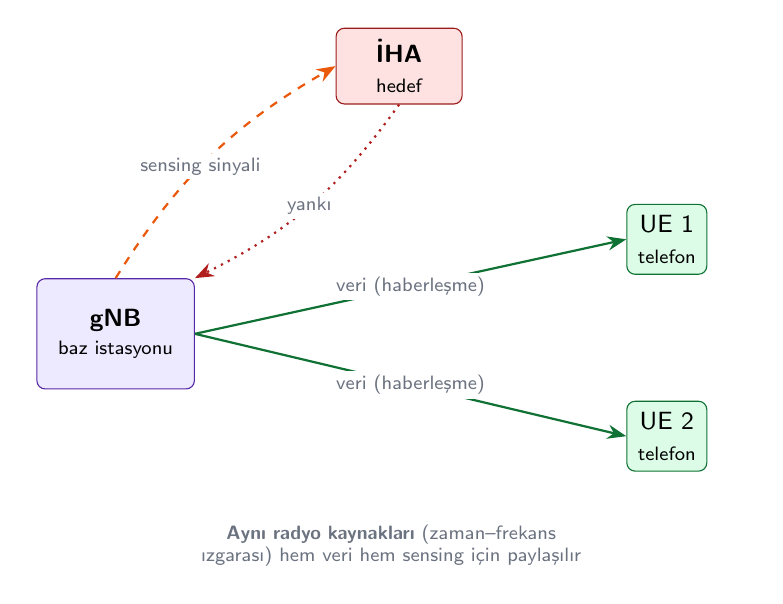
\begin{tikzpicture}[x=1cm,y=1cm]
  % gNB
  \node[ndp,minimum width=20mm,minimum height=14mm] (gnb) at (0,0) {\textbf{gNB}\\[-1pt]{\scriptsize baz istasyonu}};
  % UE'ler
  \node[ndg] (ue1) at (7.0,1.2) {UE 1\\{\scriptsize telefon}};
  \node[ndg] (ue2) at (7.0,-1.3) {UE 2\\{\scriptsize telefon}};
  % hedef
  \node[ndr,minimum width=16mm] (uav) at (3.6,3.4) {\textbf{İHA}\\{\scriptsize hedef}};
  % veri akislari
  \draw[ar,color=good!70!black] (gnb.east) -- node[lab,fill=white,inner sep=1.5pt,pos=0.5] {veri (haberleşme)} (ue1.west);
  \draw[ar,color=good!70!black] (gnb.east) -- node[lab,fill=white,inner sep=1.5pt,pos=0.5] {veri (haberleşme)} (ue2.west);
  % sensing: gonderilen sinyal ve yanki
  \draw[ar,color=warn,dashed] (gnb.north) to[bend left=14] node[lab,fill=white,inner sep=1.5pt,pos=0.45] {sensing sinyali} (uav.west);
  \draw[ar,color=bad!80!black,dotted] (uav.south) to[bend left=14] node[lab,fill=white,inner sep=1.5pt,pos=0.5] {yankı} (gnb.north east);
  \node[lab,anchor=north,text width=9cm] at (3.5,-2.3) {\textbf{Aynı radyo kaynakları} (zaman--frekans ızgarası) hem veri hem sensing için paylaşılır};
\end{tikzpicture}
\caption{ISAC fikri: gNB aynı sinyalle kullanıcılara veri taşır ve İHA'dan dönen yankıyı dinleyerek konumunu ve hızını kestirir.}
\end{figure}

\subsection{Sorun: sensing bedava değil}

Radyo kaynakları sonludur. Bir \emph{slot} içindeki bir kaynak ya bir kullanıcıya veri taşır ya da sensing sinyali olarak kullanılır.
Sensing'e ne kadar kaynak ayırırsak:
\begin{itemize}
\item \textcolor{good!70!black}{\textbf{Sensing kalitesi artar}} (daha az kaçırılan hedef, daha doğru konum),
\item \textcolor{bad!80!black}{\textbf{Haberleşme kapasitesi düşer}} (daha az throughput, daha çok gecikme).
\end{itemize}
Bu bir \textbf{ödünleşim (trade-off)}. Soru, bu ödünleşimin şeklinin ne olduğu.

\subsection{Mevcut çalışmada boşluk nerede?}

3GPP, ISAC'ı standartlaştırmak için \textbf{TR 38.765}'i (Rel-20) yazdı. Bu rapor İHA tespiti için \emph{sensing performansını} değerlendirdi:
kaçırma olasılığı, yanlış alarm, konum ve hız doğruluğu. Ama raporun kendisi şunu açıkça yazıyor
(\emph{bölüm 6.3.0}): \textit{``The performance of communication is not evaluated.''} Yani \textbf{haberleşme tarafı değerlendirilmedi}.

\begin{bulgu}[Projenin boşluğu, standardın kendi cümlesiyle]
3GPP TR 38.765 v20.0.0 bölüm 6.3.0: sensing sonuçları raporlanırken haberleşmenin etkisi \emph{hesaba katılmadı}.
Bizim katkımız tam bu eksik taraf: \textbf{sensing yükü arttıkça haberleşme ne kadar kaybediyor, ve bunu açık kaynak araçlarla nasıl ölçeriz?}
\end{bulgu}

\subsection{Üç araç, bir hikâye}

Proposal'daki üç araç bu soruya birbirini tamamlayan üç açıdan bakıyor:

\begin{figure}[H]
\centering
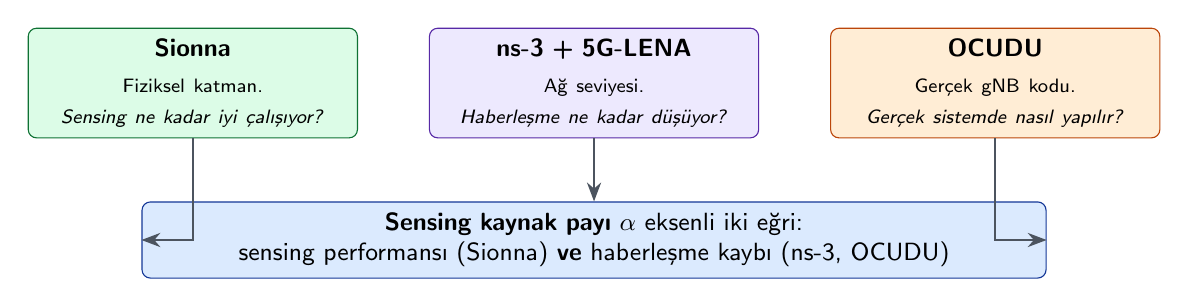
\begin{tikzpicture}[node distance=7mm and 9mm]
  \node[ndg,text width=3.9cm] (s) {\textbf{Sionna}\\[2pt]{\scriptsize Fiziksel katman.}\\{\scriptsize \emph{Sensing ne kadar iyi çalışıyor?}}};
  \node[ndp,text width=3.9cm,right=of s] (n) {\textbf{ns-3 + 5G-LENA}\\[2pt]{\scriptsize Ağ seviyesi.}\\{\scriptsize \emph{Haberleşme ne kadar düşüyor?}}};
  \node[ndw,text width=3.9cm,right=of n] (o) {\textbf{OCUDU}\\[2pt]{\scriptsize Gerçek gNB kodu.}\\{\scriptsize \emph{Gerçek sistemde nasıl yapılır?}}};
  \node[nd,text width=11.2cm,below=8mm of n] (r) {\textbf{Sensing kaynak payı $\alpha$} eksenli iki eğri:\\ sensing performansı (Sionna) \textbf{ve} haberleşme kaybı (ns-3, OCUDU)};
  \draw[ar] (s.south) |- (r.west);
  \draw[ar] (n.south) -- (r.north);
  \draw[ar] (o.south) |- (r.east);
\end{tikzpicture}
\caption{Projenin yapısı: üç araç, aynı $\alpha$ ekseninde birleşen iki sonuç.}
\label{fig:boru}
\end{figure}

\begingroup\sffamily\small
\begin{xltabular}{\textwidth}{@{}p{2.6cm}Xp{4.2cm}@{}}
\toprule
\textbf{Araç} & \textbf{Cevapladığı soru} & \textbf{Çıktısı} \\
\midrule
Sionna & Sensing sinyaline ne kadar kaynak verirsek hedefi ne kadar iyi buluruz? & Tespit ve hata eğrileri, range-Doppler haritaları \\
ns-3 + 5G-LENA & Kaynağın bir kısmı sensing'e gidince birçok kullanıcılı bir ağda throughput ve gecikme ne olur? & Throughput, gecikme, paket kaybı tabloları \\
OCUDU & Gerçek bir gNB yazılımı bu yükü nasıl zamanlar? Sensing nereye takılır? & Çalışan deney, kod haritası, tasarım önerisi \\
\bottomrule
\end{xltabular}
\endgroup

\subsection{Araştırma sorusu ve hipotezler}

\textbf{Ana soru:} Sensing için ayrılan radyo kaynağı payı $\alpha$ arttıkça, haberleşme throughput'u ve gecikmesi nasıl değişir; bu, sensing kazancıyla nasıl dengelenir?

\begin{description}[leftmargin=2.2em,labelwidth=2em,font=\sffamily\bfseries\color{acc}]
\item[H1] Haberleşme throughput'u, sensing'e giden kaynak payı kadar \emph{doğrusal} düşer: $T(\eta)=\min\{\eta,\,1-\alpha\}$.
  \textit{(Dickerson vd.~\cite{dickerson} modeli; OCUDU ölçümümüzde zaten yaklaşık olarak gördük, bkz.~Şekil~\ref{fig:ocudu-prs}.)}
\item[H2] Sensing sinyali zaman ekseninde \emph{düzensiz boşluklarla} kesildiğinde, sensing kalitesi (özellikle Doppler/hız) hızla bozulur.
  \textit{(Sionna'da basit bir deneyle gördük, bkz.~Şekil~\ref{fig:gap}.)}
\item[H3] Yüksek yükte, kaynakları sensing ve haberleşme arasında \emph{uyarlanır} paylaştıran bir politika, sabit rezervasyondan iyi bir ödünleşim verir.
  \textit{(Literatürde önerildi~\cite{dickerson}; bizim ölçmemiz gereken kısım.)}
\end{description}

\begin{dikkat}[Hipotez ne demek?]
H1--H3 \emph{kesin sonuç değil}, test edeceğimiz iddialardır. Doğru çıkabilirler de, çıkmayabilirler de. Proje başarısı, hipotezlerin doğru çıkması değil,
\textbf{iyi ölçülmüş ve açıklanmış sonuç} üretmektir.
\end{dikkat}

\section{Temel kavramlar}\label{sec:kavram}

Bu bölüm, proje boyunca duyacağınız her terimi sıfırdan anlatır. Zorlanırsanız Ek~\ref{ek:sozluk}'teki sözlüğe bakın.

\subsection{5G NR radyo kaynak ızgarası}\label{sec:grid}

5G NR'de radyo kaynağı bir \textbf{zaman--frekans ızgarasıdır}:
\begin{itemize}
\item \textbf{Zaman ekseni:} bir \textbf{slot} 14 \textbf{OFDM sembolünden} oluşur. Slot süresi alt taşıyıcı aralığına (SCS) bağlıdır:
  15\,kHz'de 1\,ms, 30\,kHz'de 0,5\,ms.
\item \textbf{Frekans ekseni:} 12 alt taşıyıcı bir \textbf{PRB}'yi (Physical Resource Block) oluşturur. 20\,MHz'lik, 15\,kHz'lik bir hücrede yaklaşık 106 PRB vardır.
\item En küçük birim \textbf{kaynak elemanı (RE)}: 1 sembol $\times$ 1 alt taşıyıcı.
\end{itemize}

Izgaranın her bölgesinin bir görevi vardır:

\begingroup\sffamily\small
\begin{xltabular}{\textwidth}{@{}p{2.2cm}X@{}}
\toprule
\textbf{Kanal/sinyal} & \textbf{Görevi} \\
\midrule
PDSCH & Kullanıcı verisi (indirme, \emph{downlink}). Throughput'u belirleyen kaynak. \\
PDCCH & Kontrol: hangi kullanıcı hangi PRB'yi alıyor? Slotun ilk sembollerinde. \\
SSB & Senkronizasyon: telefonlar hücreyi bulsun diye periyodik yayın. \\
PRS & \textbf{Konumlandırma referans sinyali} (Rel-16). Bilinen bir dizi içerir, bu yüzden \emph{radar gibi} kullanılabilir. \\
SRS & Telefonun gönderdiği (yukarı bağlantı) referans sinyali. Kanal ölçümü için. \\
\bottomrule
\end{xltabular}
\endgroup

\begin{figure}[H]
\centering
\includegraphics[width=0.88\textwidth]{sekiller/fig_grid.pdf}
\caption{Şematik kaynak ızgarası (8 slot). Turuncu bloklar slot 1 ve 5'teki sensing/PRS sinyali: kapladığı PRB'ler o slotta kullanıcı verisi için kullanılamaz.
Bu şema OCUDU'da PRS periyodu $T=4$ slot ve ofset 1 olan gerçek bir yapılandırmayı temsil eder.}
\label{fig:grid}
\end{figure}

\textbf{Sensing bu ızgarada nasıl görünür?} Sensing için gönderilen sinyal (örneğin PRS), ızgaranın bir bölgesini kaplar. Orası artık kullanıcı verisi taşıyamaz.
Ne kadar bölge kaplandığı, \textbf{sensing kaynak payı} $\alpha$'dır. Bu projenin merkezindeki sayı budur.

\subsubsection{Zihninde canlandır: ızgara bir tablodur}\label{sec:somut}

Izgarayı \textbf{bir Excel tablosu} gibi düşün: \emph{sütunlar zaman} (semboller), \emph{satırlar frekans} (alt taşıyıcılar). Scheduler bu tabloyu her slotta
\textbf{dikdörtgenlere böler}; her dikdörtgen bir kullanıcının verisidir (ya da bir sinyaldir: SSB, PRS...). Aşağıda önce tablonun ölçeğini, sonra \emph{gerçek bir gNB'nin} bu tabloyu nasıl doldurduğunu göreceksin.

\begin{figure}[H]
\centering
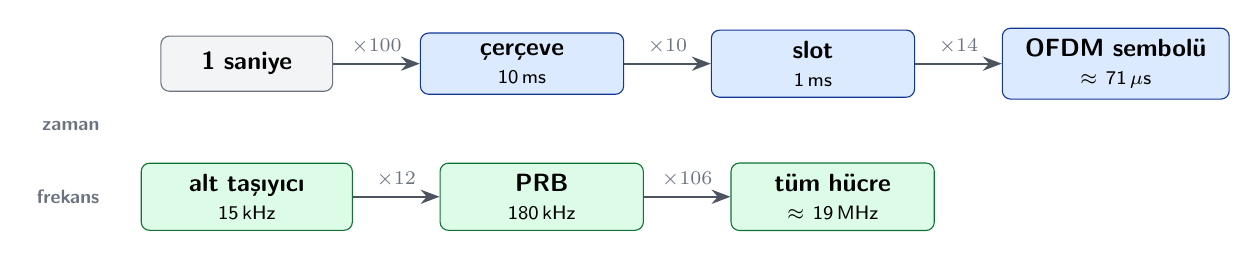
\begin{tikzpicture}[node distance=5mm and 11mm,font=\sffamily\small]
  \node[ndn,text width=1.9cm] (a) {\textbf{1 saniye}};
  \node[nd,text width=2.3cm,right=of a] (b) {\textbf{çerçeve}\\[-1pt]{\scriptsize 10\,ms}};
  \node[nd,text width=2.3cm,right=of b] (c) {\textbf{slot}\\[-1pt]{\scriptsize 1\,ms}};
  \node[nd,text width=2.6cm,right=of c] (d) {\textbf{OFDM sembolü}\\[-1pt]{\scriptsize $\approx$ 71\,$\mu$s}};
  \draw[ar] (a) -- node[lab,above] {$\times100$} (b);
  \draw[ar] (b) -- node[lab,above] {$\times10$} (c);
  \draw[ar] (c) -- node[lab,above] {$\times14$} (d);
  \node[ndg,text width=2.4cm,below=9mm of a] (e) {\textbf{alt taşıyıcı}\\[-1pt]{\scriptsize 15\,kHz}};
  \node[ndg,text width=2.3cm,right=of e] (f) {\textbf{PRB}\\[-1pt]{\scriptsize 180\,kHz}};
  \node[ndg,text width=2.3cm,right=of f] (g) {\textbf{tüm hücre}\\[-1pt]{\scriptsize $\approx$ 19\,MHz}};
  \draw[ar] (e) -- node[lab,above] {$\times12$} (f);
  \draw[ar] (f) -- node[lab,above] {$\times106$} (g);
  \node[lab,anchor=east] at ([xshift=-4mm]e.west) {\textbf{frekans}};
  \node[lab,anchor=east] at ([xshift=-4mm,yshift=9mm]e.west) {\textbf{zaman}};
\end{tikzpicture}
\caption{Zaman ve frekans eksenlerinde ``kaç tane ne'' (15\,kHz alt taşıyıcı aralığı, 20\,MHz'lik hücre). Slotun içinde 14 sütun (sembol) ve $106\times12=1272$ satır (alt taşıyıcı) vardır.}
\end{figure}

\paragraph{Bir slotun kaç kaynak elemanı var?}
\begin{equation*}
\underbrace{106}_{\text{PRB}}\times\underbrace{12}_{\text{alt taşıyıcı/PRB}}\times\underbrace{14}_{\text{sembol}}=\mathbf{17\,808}\ \text{kaynak elemanı (RE) / slot}
\end{equation*}
Saniyede 1000 slot olduğundan bu, saniyede $\approx 17{,}8$ milyon RE eder. Bir RE 64QAM ile en çok 6 bit taşıyabilir; bu yüzden teorik üst sınır slot başına $17\,808\times 6=106\,848$ bit,
yani yaklaşık 107\,Mbps'tir. Gerçek sistem bunun altında kalır, çünkü kontrol sinyalleri, referans sinyalleri ve hata düzeltme kodu yer kaplar.

\paragraph{Gerçek bir gNB bu tabloya ne yazıyor?}
OCUDU'yu çalıştırıp scheduler log'unu açtık (PRS her 4 slotta bir; \texttt{ogretici/betikler/ocudu\_slot\_log.sh}). Log'dan \emph{gerçek} iki satır:

\begin{lstlisting}
[  876.7] PDSCH: rnti=0x44 ... prb=[0, 96) symb=[1, 14) mod=64QAM ... tbs=7941
[  880.1] PUSCH: rnti=0x44 ... prb=[0, 106) symb=[0, 14) mod=64QAM ... tbs=9737
\end{lstlisting}

Bu tek satırı ``ızgara tablosu'' diliyle oku:
\begin{center}
\sffamily\small
\begin{tabularx}{\textwidth}{@{}p{3.3cm}p{4.6cm}X@{}}
\toprule
\textbf{Log'da} & \textbf{Anlamı} & \textbf{Tabloda nereye karşılık gelir?} \\
\midrule
\texttt{[ 876.7]} & Çerçeve 876, slot 7 & 876. çerçevenin (10\,ms) 8. slotu (15\,kHz'de bir çerçevede 10 slot var). \\
\texttt{prb=[0, 96)} & PRB 0'dan 95'e: \textbf{96 PRB} & Tablonun \emph{frekans} yönündeki kalınlığı: $96\times12=1152$ alt taşıyıcı. \\
\texttt{symb=[1, 14)} & Sembol 1'den 13'e: \textbf{13 sembol} & Tablonun \emph{zaman} yönündeki uzunluğu. Sembol 0 kontrol kanalına (PDCCH) kalır. \\
\texttt{mod=64QAM} & 64QAM modülasyon & Her RE 6 bit taşır (en çok). \\
\texttt{tbs=7941} & Taşıma bloğu: \textbf{7941 bayt} & Bu dikdörtgenin taşıdığı veri: $7941\times8=63\,528$ bit. \\
\bottomrule
\end{tabularx}
\end{center}

Yani bu kullanıcıya verilen dikdörtgen $96\times12\times13=\mathbf{14\,976}$ RE'dir ve $63\,528$ bit taşır:
RE başına $63\,528/14\,976\approx 4{,}24$ bit (6 bitten az, çünkü DMRS referans sinyali ve kodlama yeri tutar). Slot başına $\approx 63{,}5$\,kbit ve saniyede 1000 slot $\Rightarrow$ en çok $\approx 63{,}5$\,Mbps.

\begin{bulgu}[Throughput'u elle hesapladık, ölçümle tuttu]
Log'daki 6365 PDSCH'nin ortalama taşıma bloğu 7251 bayt, yani \textbf{58,0\,kbit/slot} (en çok kullanılan kalıp: 96 PRB, bazen 40 PRB).
\begin{itemize}[leftmargin=1.4em]
\item \textbf{PRS yokken:} saniyede 1000 PDSCH'li slot $\Rightarrow 1000\times58{,}0=58{,}0$\,Mbps. Ölçülen: \textbf{59,0\,Mbps}.
\item \textbf{PRS her 4 slotta bir iken:} saniyede 750 PDSCH'li slot $\Rightarrow 750\times58{,}0=43{,}5$\,Mbps. Ölçülen: \textbf{43,8\,Mbps}.
\end{itemize}
\textbf{Kural:} DL throughput $\approx$ (PDSCH'li slot sayısı / s) $\times$ (taşıma bloğu bit/slot). Sensing bu çarpımın birinci çarpanını (PDSCH'li slot sayısı) ya da ikincisini (PRB sayısı) küçültür. Projenin özü bu iki cümledir.
\end{bulgu}

\begin{figure}[H]
\centering
\includegraphics[width=0.98\textwidth]{sekiller/fig_slot_serit.pdf}
\caption{\textbf{Gerçek OCUDU log'undan 40 ardışık slot} (SFN 890.0'dan 893.9'a; veri: \texttt{ogretici/veri/ocudu\_slot\_serit.csv}). Her çubuk bir slotu, yüksekliği PDSCH'ye verilen PRB sayısını gösterir.
\textbf{Turuncu slotlarda PDSCH hiç yok:} bunlar 890.1, 890.5, 890.9, \ldots, yani \emph{tam her 4. slot}. PRS periyodunu 4 slot, ofsetini 1 yapmıştık.
Sarı slotlar (\texttt{.0}) yalnızca 40 PRB alıyor; muhtemelen aynı slottaki SSB yer tuttuğu için (bunu kodla doğrulamadık).}
\label{fig:slot-serit}
\end{figure}

Bu şekil bölümün en önemli görseli: \textbf{PRS'in ``kaynağı götürmesi'' soyut bir cümle değil, log'da sayılabilir bir şeydir}: her 4. slotta tablonun tamamı PRS'e gider, o slotta kullanıcıya hiçbir şey kalmaz.
Ayrıca \texttt{symb=[1, 14)} her PDSCH'de aynı: veri hep slotun \emph{tamamına} yayılıyor. Bu, Bölüm~\ref{sec:prs}'deki ``4 sembollük PRS de 12 sembollük PRS kadar kayıp veriyor'' bulgusuyla uyumlu bir açıklama olabilir
(PRS'in kapladığı PRB'lere slotun bütününde veri verilemiyor), ama bunu henüz kodla doğrulamadık.

\begin{figure}[H]
\centering
\includegraphics[width=0.96\textwidth]{sekiller/fig_izgara_kareler.pdf}
\caption{\textbf{Aynı veri, bu kez ızgara olarak:} 8 ardışık slotun her biri 14 sembol $\times$ 106 PRB'lik bir tablo. Mavi dikdörtgen log'daki PDSCH tahsisidir (\texttt{prb}, \texttt{symb} değerleri log'dan). Turuncu dikdörtgen yapılandırmadaki PRS'tir (periyot 4, ofset 1, 12 sembol, 104 PRB). Soluk yeşil şerit: PDSCH'nin başlamadığı sembol 0 (kontrol alanı). Animasyonlu hâli: \texttt{ogretici/sekiller/ocudu\_izgara\_filmi.gif}.}
\end{figure}

\begin{pilot}[Kendin dene (20 dakika)]
\begin{enumerate}[leftmargin=1.5em]
\item \textbf{Elle hesapla:} Alt taşıyıcı aralığı 15 yerine \textbf{30\,kHz}, bant 20 yerine \textbf{40\,MHz} olsun. Bu durumda PRB sayısı yine 106'dır (3GPP TS 38.101-1'deki tabloya göre; sen de tabloya bakıp doğrula, biz doğrulamadık).
  (a) Bir slot kaç ms sürer, saniyede kaç slot vardır? (b) Bir slotun RE sayısı değişir mi? (c) Saniyedeki RE sayısı kaç kat artar? (d) Bir PRB artık kaç kHz'dir?
  \emph{Beklenen cevap:} (a) 0,5\,ms, 2000 slot/s. (b) Hayır, 17\,808. (c) 2 kat ($\approx 35{,}6$ milyon RE/s). (d) $12\times30=360$\,kHz.
\item \textbf{Gerçeği gör:} Ubuntu'da \texttt{bash ogretici/betikler/ocudu\_slot\_log.sh} çalıştır. Sonra \texttt{grep -a "PDSCH: rnti" /tmp/gnb\_slotlog.log | head} ile ilk PDSCH satırlarını bul ve yukarıdaki tabloyla okumayı dene: \texttt{prb}, \texttt{symb}, \texttt{tbs} ne diyor?
\item \textbf{PRS slotlarını bul:} \texttt{grep -a "Slot decisions" /tmp/gnb\_slotlog.log | head -50} satırlarında \texttt{0 PDSCHs} geçen slotların numaralarına bak. Aralarındaki fark kaç? (Cevap: 4.)
\item \textbf{Değiştir:} \texttt{ogretici/veri/ocudu\_p4\_config.yml} dosyasında \texttt{periodicity\_slots: 8} yap, tekrar çalıştır. \texttt{0 PDSCHs} slotları şimdi kaç slotta bir? Throughput ne olur?
\end{enumerate}
\end{pilot}

\subsection{gNB'nin iç yapısı: CU, DU, RU}\label{sec:gnb}

Bir gNB tek parça değildir. Açık RAN mimarisinde (O-RAN) işlevler katmanlara bölünür:

\begin{figure}[H]
\centering
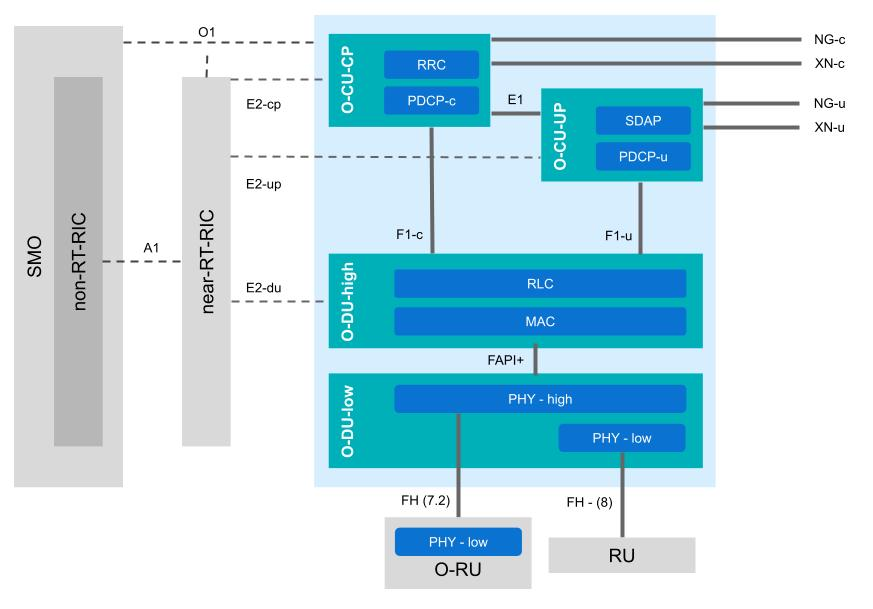
\includegraphics[width=0.78\textwidth]{sekiller/oran_gnb_arch.jpg}
\caption{O-RAN gNB mimarisi. Kaynak: OCUDU deposu, \texttt{lib/oran\_gnb\_arch.jpg} (SPDX: BSD-3-Clause-Open-MPI, Software Radio Systems Limited).
Biz özellikle \textbf{O-DU-high} içindeki \textbf{MAC} (scheduler orada) ve \textbf{O-DU-low}'daki \textbf{PHY} ile ilgileniyoruz.}
\label{fig:oran}
\end{figure}

\begingroup\sffamily\small
\begin{xltabular}{\textwidth}{@{}p{2.3cm}X@{}}
\toprule
\textbf{Parça} & \textbf{Ne yapar?} \\
\midrule
CU-CP / CU-UP & Merkezi birim: kontrol düzlemi (RRC, bağlantı yönetimi) ve kullanıcı düzlemi (veri yönlendirme, SDAP/PDCP). Çekirdek ağla konuşur. \\
DU-high & RLC ve \textbf{MAC}. MAC'in içindeki \textbf{scheduler}, her slotta kaynakları kullanıcılara dağıtır. \\
DU-low & PHY (fiziksel katman): modülasyon, kodlama, FFT. PRS sinyalini üreten kod burada. \\
RU & Radyo: antenler ve RF. Bizde gerçek RU yok; yazılımla taklit ediliyor (\texttt{ru\_dummy}, ZMQ). \\
\bottomrule
\end{xltabular}
\endgroup

\subsection{Scheduler: slotta kim ne alır?}\label{sec:sched}

\textbf{Scheduler}, \emph{her slotta} (örneğin her 1\,ms) bir karar verir: hangi kullanıcı hangi PRB'leri, hangi modülasyonla alacak?
Bu kararın sonucu bir ``tahsis listesi''dir. Çok kullanıcılı bir ağda throughput'u ve gecikmeyi esas olarak scheduler belirler.

Yaygın politikalar:
\begin{itemize}
\item \textbf{Round-Robin (RR):} herkese sırayla.
\item \textbf{Proportional Fair (PF):} kanalı iyi olana öncelik verir ama kimseyi aç bırakmaz. En yaygın politika.
\item \textbf{QoS-farkında (örn.\ M-LWDF, EXP/PF):} gecikme bütçesi yaklaşan paketlere öncelik. (Capozzi vd.~\cite{capozzi}'nin taraması bu aileyi anlatır.)
\end{itemize}

\textbf{Neden önemli?} Sensing sinyali, scheduler'ın dağıtabileceği kaynak havuzundan düşer. Yani sensing bir \emph{scheduler problemi}dir:
sensing kaynaklarını önceden mi ayırırız, yoksa yük arttıkça mı küçültürüz?

\subsection{OFDM radar: yankıdan menzil ve hız}\label{sec:radar}

OFDM sinyali (5G'nin kullandığı) bir radar olarak da çalışır. Fikir şu:

\begin{enumerate}
\item gNB bilinen bir OFDM sinyali gönderir ($X$).
\item Hedeften yansıyan sinyal ($Y$) gecikmiş ve Doppler kaymış olarak geri gelir.
\item $H = Y/X$ (kanal tahmini) hesaplanır. Alt taşıyıcılar arasındaki \textbf{faz eğimi gecikmeyi (menzili)}, semboller arasındaki \textbf{faz eğimi Doppler'i (hızı)} verir.
\item Bir \textbf{2 boyutlu FFT} bu iki eğimi bir \textbf{range-Doppler haritasına} çevirir. Hedef haritada bir tepe noktası olarak görünür.
\end{enumerate}

\begin{figure}[H]
\centering
\includegraphics[width=0.78\textwidth]{sekiller/fig_rd_map.pdf}
\caption{\textbf{Simülasyon:} iki hedefli (120\,m, +25\,m/s ve 260\,m, $-18$\,m/s) bir OFDM radarın range-Doppler haritası.
Parametreler TR 38.765 Ek~A ile uyumlu: 4,9\,GHz, 30\,kHz SCS, 1024 alt taşıyıcı ($\approx$ 30,7\,MHz), 128 sembol. Halkalar gerçek konumdur; tepeler halkaların içine düşer.
Betik: \texttt{ogretici/betikler/make\_figs.py}.}
\label{fig:rd}
\end{figure}

\textbf{Çözünürlük}, iki hedefi ayırt etme yeteneğidir ve iki şeye bağlıdır:
\begin{equation}
\Delta R=\frac{c}{2W},\qquad \Delta v=\frac{\lambda}{2\,M\,T_{sym}}
\end{equation}
$W$: sensing sinyalinin bant genişliği, $M$: gözlenen OFDM sembol sayısı, $T_{sym}$: sembol süresi, $\lambda$: dalga boyu.
Bu denklemler Lin~\cite{lin}'in IV.\ bölümünde ve Dickerson vd.~\cite{dickerson}'in Tablo~II'sinde de geçer.

\begin{figure}[H]
\centering
\includegraphics[width=0.92\textwidth]{sekiller/fig_resolution.pdf}
\caption{Çözünürlük, sensing'e verdiğimiz kaynakla belirlenir. \textbf{Daha çok bant ($W$) $\rightarrow$ daha ince menzil.
Daha çok sembol ($M$) $\rightarrow$ daha ince hız.} Bu yüzden ``sensing'e kaynak vermek'' sensing kalitesinin doğrudan sebebidir.}
\end{figure}

\begin{pilot}[Kendi gözünle gör]
\texttt{kurulum\textbackslash sionna\_dogrulama.py} dosyasını çalıştırın. Gerçek hedef 120\,m ve 25\,m/s'ydi; betik hedefi 122,1\,m ve 25,9\,m/s olarak buldu.
Hata, çözünürlük hücresinin (4,88\,m, 6,47\,m/s) içinde. \textbf{Soru:} bant genişliğini 4~kat artırsak menzil hatası ne olur? (Cevap: yaklaşık 4~kat azalır, formülden.)
\end{pilot}

\subsection{Sensing sinyali olarak ne kullanılır?}\label{sec:sinyal}

Sensing için yeni bir sinyal icat etmek yerine, 5G'de zaten olan ve alıcının \emph{önceden bildiği} sinyaller kullanılır
(bilinen bir sinyal olmazsa $H=Y/X$ hesaplanamaz):

\begingroup\sffamily\small
\begin{xltabular}{\textwidth}{@{}p{2cm}XX@{}}
\toprule
\textbf{Sinyal} & \textbf{Avantaj} & \textbf{Sorun} \\
\midrule
PRS (DL) & Geniş bant, seyrek yapılandırılabilir, standart (Rel-16). Radar için en çok çalışılan aday \cite{wei,nist,khos}. & Comb yapısı \emph{hayalet hedef (ghost target)} üretebilir \cite{khos}. \\
DMRS (DL, PDSCH içinde) & Veri sinyaliyle birlikte gelir: sensing neredeyse bedava. & Seyrek, yalnızca veri olan yerde var. \\
SRS (UL) & Telefon gönderir; bistatic/pasif sensing mümkün \cite{gurung}. & Telefonun gücü ve zamanlaması sınırlı. \\
Özel sinyal (örn.\ ZC) & Tasarım serbest, iyi korelasyon. & Standartta yok; ek kaynak ister \cite{dickerson}. \\
\bottomrule
\end{xltabular}
\endgroup

\textbf{OCUDU'da PRS zaten var} (Bölüm~\ref{sec:ocudu}): hem MAC'te zamanlayıcısı hem PHY'de üretici kodu mevcut. Bu, projenin en önemli teknik bulgularından biridir.

\subsection{Metrikler: neyi ölçüyoruz?}\label{sec:metrik}

İki taraf için iki metrik ailesi:

\begingroup\sffamily\small
\begin{xltabular}{\textwidth}{@{}p{3.1cm}Xp{3.2cm}@{}}
\toprule
\textbf{Taraf} & \textbf{Metrik} & \textbf{Nereden?} \\
\midrule
\multirow{4}{*}{Sensing}
 & Kaçırma olasılığı $P_{md}$ (hedef var, bulunamadı) & TR 38.765 \S4.1 \\
 & Yanlış alarm Tip~1 $P_{f1}$ (hedef yok, tespit var) & TR 38.765 \S4.1 \\
 & Yanlış alarm Tip~2 $P_{f2}$ (tespit var, ama gerçek hedefle eşleşmiyor) & TR 38.765 \S4.1 \\
 & Yatay/dikey konum hatası, hız hatası & TR 38.765 \S4.1 \\
\midrule
\multirow{3}{*}{Haberleşme}
 & Throughput, gecikme, paket kaybı, adalet (fairness) & Capozzi vd.\ \cite{capozzi} \S V \\
 & Kaynak kullanımı & ns-3, OCUDU çıktıları \\
\midrule
Ödünleşim & \textbf{Sensing kaynak oranı} $\alpha$ (Tip~1,2,3 kaynaklar, Seçenek~1 ve~2) & TR 38.765 \S6.2 \\
\bottomrule
\end{xltabular}
\endgroup

TR~38.765'in hedefleri (Tablo~4.2-1): $P_{md}$, $P_{f1}$, $P_{f2}\leq\%5$, yatay ve dikey konum hatası 10\,m (\%90 güvenle), hız hatası 5\,m/s (\%90 güvenle).
Bu eşikler, sensing tarafında ``yeterince iyi''nin ne demek olduğunu söyler.

\section{3GPP standartları: ne söylüyorlar, biz neyi alıyoruz?}\label{sec:3gpp}

\subsection{3GPP nedir, bu projede neden önemli?}

\textbf{3GPP}, mobil ağ standartlarını yazan kuruluştur. 5G'nin her özelliği ``Release'' (sürüm) adı altında sürümlenir. Bu projede standart üç iş yapar:
\begin{enumerate}
\item Sensing için \textbf{ne ölçüleceğini} (metrikler) ve \textbf{hangi eşiklerin} yeterli sayılacağını söyler.
\item Simülasyonda hangi \textbf{senaryo ve parametreleri} kullanacağımızı verir (ki sonuçlarımız literatürle karşılaştırılabilsin).
\item Sensing'in ağ mimarisinde \textbf{nereye oturacağını} tarif eder (SenF, NsAP).
\end{enumerate}

\subsection{ISAC'ın standartlardaki yolculuğu}

\begin{figure}[H]
\centering
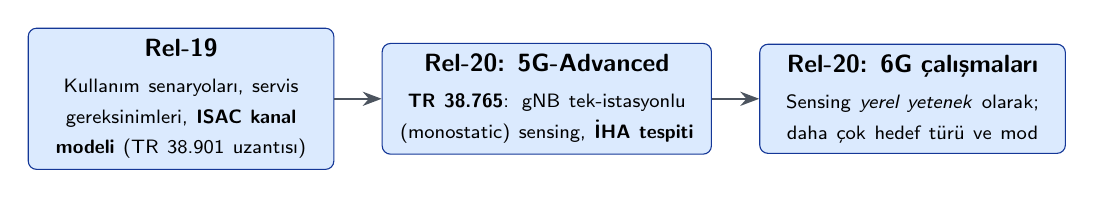
\begin{tikzpicture}[node distance=6mm and 6mm]
  \node[nd,text width=3.6cm] (r19) {\textbf{Rel-19}\\[2pt]{\scriptsize Kullanım senaryoları, servis gereksinimleri, \textbf{ISAC kanal modeli} (TR~38.901 uzantısı)}};
  \node[nd,text width=3.9cm,right=of r19] (r20a) {\textbf{Rel-20: 5G-Advanced}\\[2pt]{\scriptsize \textbf{TR~38.765}: gNB tek-istasyonlu (monostatic) sensing, \textbf{İHA tespiti}}};
  \node[nd,text width=3.6cm,right=of r20a] (r20b) {\textbf{Rel-20: 6G çalışmaları}\\[2pt]{\scriptsize Sensing \emph{yerel yetenek} olarak; daha çok hedef türü ve mod}};
  \draw[ar] (r19) -- (r20a);
  \draw[ar] (r20a) -- (r20b);
\end{tikzpicture}
\caption{ISAC'ın 3GPP'deki gelişimi. Kaynak: Lin \cite{lin,lin20}.}
\end{figure}

\textbf{Biz Rel-20 / 5G-Advanced hattındayız:} gNB'nin kendi sinyalini kullanarak (tek istasyon) İHA tespiti. Proposal'ın başvurduğu referans da budur.

\subsection{TR 38.765'e rehber (v20.0.0, 2026-06)}

Tüm raporu okumanıza gerek yok. Şu tablo hangi bölümde ne olduğunu ve neden önemli olduğunu söyler:

\begingroup\sffamily\small
\begin{xltabular}{\textwidth}{@{}p{1.5cm}p{4.9cm}X@{}}
\toprule
\textbf{Bölüm} & \textbf{İçerik} & \textbf{Bizim için önemi} \\
\midrule
4.1 & Performans metrikleri ve formülleri ($P_{md}$, $P_{f1}$, $P_{f2}$, konum/hız hatası) & Sensing metriklerimizi \emph{buradan alırız}; kendi tanımımızı uydurmayız. \\
4.2 & Hedefler: $P_{md}, P_{f1}, P_{f2} \leq \%5$; 10\,m ve 5\,m/s (\%90) & Sensing ``yeterince iyi'' eşiği. \\
\textbf{6.2} & \textbf{Sensing kaynak oranı:} Tip~1/2/3 kaynaklar, Seçenek~1 ve~2 & \textbf{Overhead'i nasıl tanımlayacağımızın standart cevabı.} \\
6.2, Tablo 6.2-1 & Baseline~1 (52\,dBm, 80\,dB izolasyon), Baseline~2 (37\,dBm, 65\,dB) & Simülasyonda kullanacağımız referans senaryolar. \\
5 & Ölçüm raporlama seviyeleri A, B, C, D & Sensing verisinin ağ taşıma yükünü hesaplamak için. \\
7--8 & Ağ mimarisi: SenF, NsAP, sensing başlatma/rapor prosedürleri & OCUDU'da sensing'in nereye takılacağı. \\
9 & Sonuç: Seviye~A desteklenmedi, Seviye~C kabul, SCTP tabanlı protokol & Tasarım kararlarını gerekçelendirmek için. \\
Ek A & Değerlendirme varsayımları & Simülasyon parametre tablosu. \\
\bottomrule
\end{xltabular}
\endgroup

\subsubsection{Değerlendirme senaryosu (Ek A)}

\begingroup\sffamily\small
\begin{xltabular}{\textwidth}{@{}p{4.8cm}X@{}}
\toprule
\textbf{Parametre} & \textbf{Değer} \\
\midrule
Senaryo & UMa-AV (şehir makro hücresi, hava aracı hedefi), ikili mesafe 500\,m \\
Taşıyıcı / bant / SCS & 4 veya 4,9\,GHz (FR1) / 100\,MHz / 30\,kHz \\
Yerleşim & 7 makro site, her sitede 3 sektör \\
Anten (gNB) & 8$\times$8$\times$2 eleman, Tx ve Rx \\
gNB gücü & 37 veya 52\,dBm \\
Anten izolasyonu (Tx $\rightarrow$ Rx) & 65 veya 80\,dB \\
Hedef & Küçük İHA (0,3$\times$0,4$\times$0,2\,m), sektör başına $N=5$, yükseklik 25--300\,m, yatay hız 0--180\,km/s \\
Sensing modu & gNB tek istasyon (monostatic), \textbf{Tx ve Rx aynı anda çalışır} \\
Öz-girişim (self-interference) & Artık sızıntı gürültü olarak modellenir ($-94+X$\,dBm, 100\,MHz'de) \\
\bottomrule
\end{xltabular}
\endgroup

\begin{dikkat}[Öz-girişim: monostatic sensing'in en zor kısmı]
Aynı gNB hem gönderip hem dinlediği için kendi vericisinin sızıntısı, İHA'dan dönen çok zayıf yankıdan \emph{birçok büyüklük mertebesi} (orders of magnitude) güçlü olabilir \cite{lin}. Bu yüzden standart,
anten izolasyonunu (65 veya 80\,dB) ve artık sızıntıyı değerlendirmenin \emph{parçası} yapıyor. Lin~\cite{lin} bunu IV.B bölümünde ``monostatic gNB sensing'in tanımlayıcı zorluğu'' diye anlatır.
Bizim ns-3 ve OCUDU çalışmamız öz-girişimi modellemez; yalnızca \emph{kaynak tüketimine} bakar. Bunu raporda açıkça sınırlılık olarak yazmalıyız.
\end{dikkat}

\subsubsection{Sensing kaynak oranı (Bölüm 6.2): bizim ana metriğimiz}

Standart üç tür kaynak tanımlar:
\begin{itemize}
\item \textbf{Tip~1:} sensing sinyali için kullanılan kaynaklar.
\item \textbf{Tip~2:} Tip~1'in, aynı zamanda haberleşme için de kullanılan kısmı (olmayabilir).
\item \textbf{Tip~3:} sensing sinyali taşımayan ama sensing işlemi yüzünden haberleşmeye de açılamayan kaynaklar.
\end{itemize}
İki seçenekle oran hesaplanır (hepsi tüm DL+UL kaynaklarına bölünür):
\begin{equation}
\text{Seçenek 1: }\ \frac{T_1+T_3}{\text{toplam}},\qquad \text{Seçenek 2: }\ \frac{T_1-T_2+T_3}{\text{toplam}}
\end{equation}
Tip~2 yoksa iki seçenek aynıdır. Biz ilk aşamada bunu kullanırız: OCUDU'daki PRS rezervasyonu Tip~1'dir (veri taşımaz, Tip~2 yok) ve Tip~3'ü de gözleyebiliriz (Bölüm~\ref{sec:ocudu}'daki ``kaybolan slot'' bulgusu tam olarak bir Tip~3 benzeri etkidir).

\subsubsection{Ölçüm raporlama seviyeleri (Bölüm 5)}

Sensing sonuçları gNB'den çekirdek ağdaki sensing işlevine \emph{ne ayrıntıda} gönderilir? Ayrıntı arttıkça taşıma yükü artar:

\begingroup\sffamily\small
\begin{xltabular}{\textwidth}{@{}p{1.5cm}Xp{2.2cm}p{3.2cm}@{}}
\toprule
\textbf{Seviye} & \textbf{İçerik} & \textbf{Taşıma yükü} & \textbf{TR 38.765 kararı} \\
\midrule
A & Ham veri (anten başına, sembol başına kanal tahmini) & Çok yüksek & \textbf{Desteklenmedi} \\
B & Gecikme/Doppler/açı profilleri & Yüksek & Değerlendirildi \\
C & \textbf{Tespit edilen yol/nokta başına} (menzil, hız, açı, güç, güven) & Orta & \textbf{İleri normatif çalışma için kabul} \\
D & Nesne seviyesi (konum, hız, sınıf, iz kimliği) & Düşük & Gizlilik/güvenlik çözülürse \\
\bottomrule
\end{xltabular}
\endgroup
Lin~\cite{lin} Tablo~2 aynı dört soyutlamayı (örnek, profil, tespit noktası, nesne) ``transport yükü'' ve ``füzyon'' açısından karşılaştırır.

\subsection{Mimari: SenF ve NsAP}\label{sec:senf}

Rel-20 mimarisi, çekirdek ağa yeni bir mantıksal işlev ekler: \textbf{SenF (Sensing Function)}. Görevleri: sensing servisini yetkilendirmek, sensing yapacak gNB'yi seçmek, parametreleri vermek, ölçümleri toplamak ve dış uygulamalara sunmak \cite{lin}.
gNB ile SenF arasındaki konuşma için ise yeni bir protokol önerilir: \textbf{NsAP}.

\begin{figure}[H]
\centering
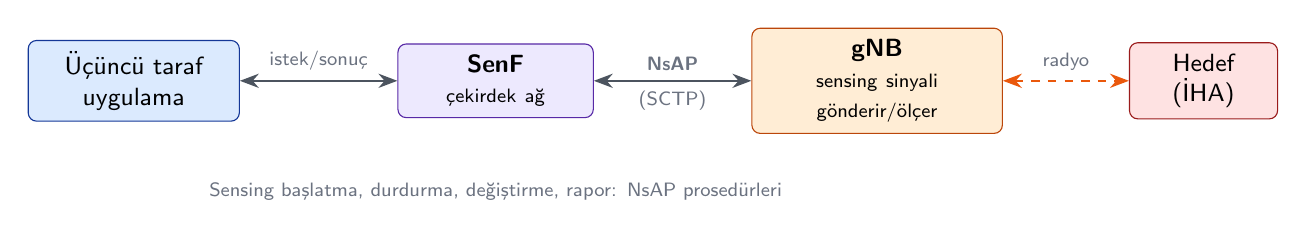
\begin{tikzpicture}[node distance=8mm and 20mm]
  \node[nd,text width=2.4cm] (af) {Üçüncü taraf\\uygulama};
  \node[ndp,text width=2.2cm,right=of af] (senf) {\textbf{SenF}\\{\scriptsize çekirdek ağ}};
  \node[ndw,text width=2.9cm,right=of senf] (gnb) {\textbf{gNB}\\{\scriptsize sensing sinyali gönderir/ölçer}};
  \node[ndr,text width=1.6cm,right=16mm of gnb] (uav) {Hedef\\(İHA)};
  \draw[dar] (af) -- node[lab,above] {istek/sonuç} (senf);
  \draw[dar] (senf) -- node[lab,above] {\textbf{NsAP}} node[lab,below] {(SCTP)} (gnb);
  \draw[dar,dashed,color=warn] (gnb) -- node[lab,above] {radyo} (uav);
  \node[lab,below=7mm of senf,text width=8cm] (n1) {Sensing başlatma, durdurma, değiştirme, rapor: NsAP prosedürleri};
\end{tikzpicture}
\caption{Rel-20 ISAC mimarisinin sadeleştirilmiş görünümü (TR 38.765 bölüm 7--8; Lin \cite{lin} bölüm III.A).}
\end{figure}

NsAP prosedürleri (TR 38.765 bölüm 8): \textbf{Sensing Initiation} (istek/cevap/hata), \textbf{SenF-initiated Sensing Abort}, \textbf{SenF-initiated Sensing Modification},
\textbf{gNB-initiated Sensing Failure indication}, \textbf{Sensing Report}; yönetim tarafında \textbf{Ns Setup}, \textbf{RAN Configuration Update}, \textbf{Error indication}.
Sensing verisi için üç protokol yığını değerlendirildi; \textbf{SCTP tabanlı olanı (Seçenek~1)} önerildi.

\textbf{Bizim için anlamı:} OCUDU gerçek bir 5G gNB uygulamasıdır; NsAP gibi bir arayüz henüz yok. Bunu eklemek ``tam bir sensing özelliği'' olurdu,
ama proje kapsamı için fazla büyük. Biz bunu \emph{tasarım seviyesinde} (bir diyagram ve bir arayüz taslağı) ele alacağız, kodlamayı değil.

\subsection{Kanal modeli: hedef, arka plan ve yerel kuplaj}

Rel-19, TR~38.901'e \emph{sensing'e özgü} bir uzantı ekledi \cite{lin,liu19}. Fikir: bir sensing kanalı üç parçaya ayrılır:
\begin{itemize}
\item \textbf{Hedef kanalı:} gNB $\rightarrow$ hedef $\rightarrow$ gNB yolu ve hedefin yansıtma özelliği (RCS).
\item \textbf{Arka plan kanalı:} bina, ağaç, araba gibi \emph{hedef olmayan} yansıtıcılar (clutter).
\item \textbf{Yerel kuplaj:} vericiden alıcıya doğrudan sızıntı (öz-girişim).
\end{itemize}
Ayrıca RCS sabit bir sayı değil; açıya, polarizasyona ve frekansa göre değişir. Bir İHA, yalnızca biraz konum değiştirince RCS çukurlarına girip \emph{kaybolabilir} \cite{lin}.

\subsection{Hangi standart belgelerini bilmeliyiz?}

\begingroup\sffamily\small
\begin{xltabular}{\textwidth}{@{}p{2.7cm}X@{}}
\toprule
\textbf{Belge} & \textbf{Ne için} \\
\midrule
TR 38.765 & ISAC çalışması, \textbf{ana referansımız} (indirildi, \texttt{makaleler/} klasöründe). \\
TR 38.901 & Kanal modeli; Rel-19 ISAC uzantısı (hedef/arka plan kanalı). \\
TS 38.211 \S7.4.1.7 & \textbf{PRS sinyalinin tanımı} (OCUDU kodundaki yorumlarda bu bölüme atıf var). \\
TS 38.455 \S9.2.44 & PRS kaynak kümesi yapılandırması (NRPPa); OCUDU'nun PRS parametreleri bunu izler. \\
TR 36.777 & İHA kanal modeli (TR 38.765 Ek~A bu belgenin B.1.3 maddesine atıf yapar). \\
\bottomrule
\end{xltabular}
\endgroup

\begin{ipucu}[Standart belgesi nasıl okunur?]
Standartlar roman değil, \emph{başvuru} metinleridir. Baştan sona okumayın. \textbf{(1)} İçindekilerden ihtiyacınız olan bölümü bulun, \textbf{(2)} tanımları ve tablolardaki sayıları okuyun,
\textbf{(3)} ``NOTE'' kutularına özellikle bakın, çünkü kısıtlar ve belirsizlikler orada yazılıdır. TR 38.765'te de projenin boşluğunu gösteren cümle bir bölüm girişinde duruyordu.
\end{ipucu}

\section{Üç araç: ne işe yarar, biz ne yaptırırız?}\label{sec:arac}

\subsection{Sionna: fiziksel katman ve ray tracing}\label{sec:sionna}

\textbf{Sionna}, NVIDIA'nın açık kaynak, TensorFlow tabanlı fiziksel katman kütüphanesidir \cite{sionna}. İki parçası var:
\begin{itemize}
\item \textbf{Sionna (çekirdek):} OFDM, MIMO, kanal kodlama, kanal modelleri (bit hata oranı eğrileri gibi bağlantı seviyesi simülasyon).
\item \textbf{Sionna RT:} 3B bir sahnede (bina, yol) ışın izleme ile \emph{gerçek yer-özel} kanal üretir \cite{sionnart}. Sahnede bir verici ve alıcı koyup hangi yolların oluştuğunu hesaplar.
\end{itemize}

\textbf{Projedeki rolü:} sensing'in \emph{ne kadar iyi} çalıştığını göstermek. Yani şu eğriyi çıkarmak: ``sensing'e ayrılan bant genişliği ve sembol sayısı arttıkça menzil/hız doğruluğu ve tespit olasılığı nasıl değişir?''
Bunun ilk adımını Bölüm~\ref{sec:radar}'de zaten attık (range-Doppler haritası, çözünürlük). Resmî Sionna RT öğreticileri: \emph{Introduction to Sionna RT}, \emph{Tutorial on Mobility},
\emph{Tutorial on Radio Maps}, \emph{Tutorial on Radar Cross Section (RCS)}.

\begin{bulgu}[Sionna ile ilgili iki tuzak (ölçülen)]
\textbf{(1)} Python 3.11'de \texttt{pip install sionna} en yeni sürümü, \textbf{Sionna 2.2.0}'ı seçiyor (kurulum sırasında PyTorch indirdi; yani muhtemelen farklı bir API, bunu incelemedik). Betiklerimiz 1.2.2 için yazıldığından \texttt{sionna==1.2.2} sabitliyoruz.
\textbf{(2)} Sionna RT, Windows'ta CPU üzerinde çalışmak için \textbf{LLVM} ister; yoksa \texttt{LLVM-C.dll bulunamadı} hatası verir (\texttt{kurulum/03-sionna-windows.md} bölüm 5).
\end{bulgu}

\subsubsection{Haberleşme zamanlaması sensing'i bozar mı? (basit deney)}

Haberleşme scheduler'ı, sensing sinyalinin bazı OFDM sembollerini başka kullanıcılara verirse, sensing alıcısı sembol dizisinde \emph{boşluklar} görür.
Lin~\cite{lin} bunu şöyle özetler: ``sensing fırsatları arasındaki boşluklar Doppler işlemeyi bozar''. Bunu tek hedefli bir OFDM radarla denedik:

\begin{figure}[H]
\centering
\includegraphics[width=0.78\textwidth]{sekiller/fig_gap.pdf}
\caption{\textbf{Simülasyon (basit model, 12 koşunun ortalaması):} OFDM sembollerinin yüzde kaçı sensing'e kullanılamıyorsa range-Doppler haritasında tepe/yan lob oranı (ne kadar yüksekse o kadar iyi) nasıl düşüyor?
Rastgele dağılmış boşluklar, aynı oranda ardışık boşluktan \emph{daha çok} zarar veriyor.}
\label{fig:gap}
\end{figure}
\begin{figure}[H]
\centering
\includegraphics[width=0.95\textwidth]{sekiller/fig_gap_maps.pdf}
\caption{Aynı deneyden haritalar. Boşluk arttıkça hedefin etrafında hız ekseni boyunca \emph{sahte yan loblar} oluşur; hedefin gerçek hızı bulanıklaşır.}
\end{figure}

\begin{dikkat}[Bu bir oyuncak model]
Bu deney \emph{tek hedef, sabit SNR, ideal kanal, gerçekçi olmayan boşluk dağılımları} ile yapıldı. Sonucun \emph{yönü} (boşluk $\rightarrow$ kötüleşme) literatürle uyumludur,
ama sayıları (dB) gerçek bir sistem için geçerli değildir. Raporda bu deneyi ``kavramı gösteren simülasyon'' olarak sunun, ``sonuç'' olarak değil.
\end{dikkat}

\subsection{ns-3 ve 5G-LENA: ağ seviyesi simülasyon}\label{sec:ns3}

\textbf{ns-3}, ayrık olay tabanlı bir ağ simülatörüdür. \textbf{5G-LENA} (\texttt{nr} modülü) onun üstüne eklenen 5G NR modülüdür: gerçek protokol yığınını (PHY, MAC, RLC, PDCP, çekirdek ağ) 3GPP'ye uygun olarak simüle eder \cite{lena}.
Kalibrasyonu 3GPP referans sonuçlarına karşı yapılmıştır \cite{koutlia}. Büyük bir avantajı: \emph{çok kullanıcılı} bir ağda scheduler etkisini görebilmemiz.

\textbf{Nasıl çalışır?} Bir C++ senaryo dosyası (``örnek'') düğümleri, anten dizilerini, bantları ve trafik akışlarını tanımlar; simülatör çalışır ve her akış için throughput, gecikme, jitter ve paket sayılarını yazar.

\begin{figure}[H]
\centering
\includegraphics[width=0.95\textwidth]{sekiller/term_ns3.pdf}
\caption{Gerçek çıktı: \texttt{./ns3 run "cttc-nr-demo --ueNumPergNb=5"} komutunun son satırları (Ubuntu/WSL2). Her akış için throughput, gecikme, jitter ve alınan paket sayısı.}
\end{figure}

\begin{bulgu}[ns-3 ölçümü: UE sayısına göre throughput ve gecikme]
\texttt{cttc-nr-demo} örneğini \texttt{--ueNumPergNb} = 1, 2, 5, 10, 20 ile çalıştırdık (5G-LENA v5.1, ns-3.48, 1\,s simülasyon, tek koşu). Sonuçlar:\par
\begin{center}
\sffamily\small
\begin{tabular}{@{}rrrr@{}}
\toprule
UE/gNB & akış & toplam throughput (Mbps) & ort.\ gecikme (ms) \\
\midrule
1 & 1 & 10,2 & 0,28 \\
2 & 2 & 112,5 & 0,59 \\
5 & 5 & 219,7 & 9,97 \\
10 & 10 & 238,3 & 57,9 \\
20 & 20 & 288,2 & 123,6 \\
\bottomrule
\end{tabular}
\end{center}
\textbf{Yorum:} Örnek, UE'leri iki gruba böler: bir kısmına düşük gecikmeli 10,24\,Mbps trafik, kalanına 102,4\,Mbps ``best effort'' trafik verir (5 UE'de çıktıda 3'üne 10,24 ve 2'sine 102,4\,Mbps verildiğini gördük).
Yük arttıkça toplam kapasite doygunluğa varır ve gecikme patlar.
Bu, \emph{kaynaklar azalırsa} ne olacağının bir önizlemesidir: sensing de benzer şekilde kapasite alır.
\end{bulgu}

\begin{figure}[H]
\centering
\includegraphics[width=0.92\textwidth]{sekiller/fig_ns3_ues.pdf}
\caption{Yukarıdaki tablo grafik olarak (gerçek 5G-LENA ölçümü; veri: \texttt{ogretici/veri/ns3\_ue\_sweep.csv}).}
\end{figure}

\subsubsection{Analitik model: sensing kaynak payı ve throughput}

Dickerson vd.~\cite{dickerson}, sensing'in kaynak tüketimini şöyle modeller (denklem 9--12):
\begin{equation}
\alpha_{sense}=\frac{N_b}{1-OH}\cdot\frac{f_{sense}}{N_{sym/sn}}\cdot\frac{N_{PRB,sense}}{N_{PRB,toplam}},\qquad
T(\eta)=\min\{\eta,\;1-\alpha_{sense}\}
\end{equation}
$N_b$: sensing ışın sayısı, $f_{sense}$: saniyedeki sensing sayısı, $N_{PRB,sense}$: bir sensing dalga biçiminin kapladığı PRB, $OH$: sabit NR kontrol yükü,
$\eta$: sunulan haberleşme yükü (normalize).

Makalenin parametreleriyle ($N_{PRB,toplam}=270$, $OH=0{,}14$, 14\,000 sembol/s, $N_{ZC}=1291\Rightarrow108$ PRB, $f_{sense}=500$\,Hz) \textbf{makalenin verdiği iki sayıyı elle yeniden hesapladık}:
tek ışın için $\alpha=\%1{,}66$ ve sekiz ışın için $\alpha=\%13{,}29$ (makalede de aynı değerler).

\begin{figure}[H]
\centering
\includegraphics[width=0.98\textwidth]{sekiller/fig_d1_model.pdf}
\caption{Dickerson vd.\ modelinin yeniden üretimi. Sol: sensing hızı arttıkça kaynak payı. Sağ: sunulan throughput. 8 ışında yüksek yükte throughput \%86,7'de tavan yapar.}
\end{figure}

\subsubsection{5G-LENA'ya sensing yükünü nasıl koyarız? (açık tasarım sorusu)}\label{sec:ns3tasarim}

5G-LENA'da hazır bir sensing modeli \textbf{yok}. Sensing yükünü simülasyonda temsil etmenin üç aday yolu var; hangisinin \emph{mümkün ve yeterince doğru} olduğunu \textbf{pilot görev} cevaplayacak:

\begingroup\sffamily\small
\begin{xltabular}{\textwidth}{@{}p{0.4cm}p{4.0cm}XX@{}}
\toprule
 & \textbf{Yol} & \textbf{Artısı} & \textbf{Riski} \\
\midrule
a & Bant genişliğini $(1-\alpha)$ ile küçült & Çok basit, kodlama yok & Sensing'in ``zamansal'' yapısını (periyodik, atımlı) hiç temsil etmez \\
b & Sensing'i yüksek öncelikli periyodik bir trafik akışı olarak ekle & Atımlı yapı ve scheduler etkisi görünür & Gerçek PRB rezervasyonu değil, trafik: yaklaşım \\
c & Scheduler'ı değiştirip PRB'leri periyodik rezerve et & En gerçekçi (OCUDU'daki PRS gibi) & C++ içinde geliştirme ister; en çok emek \\
\bottomrule
\end{xltabular}
\endgroup

Önerimiz önce \textbf{(a) ve (b)} ile başlamak ve \textbf{(c)'yi, OCUDU ölçümüyle (Bölüm~\ref{sec:ocudu}) tutarlılık kontrolü olarak} ancak zaman kalırsa denemek.

\subsubsection{Sionna'dan ns-3'e kanal köprüsü: SioLENA}

Ropitault vd.~\cite{siolena}, Sionna RT'nin ürettiği çok yollu kanalı (gecikme, genlik, faz, açı) CSV olarak alıp 5G-LENA'nın kanal modeline besleyen \textbf{SioLENA} modülünü yayımladı
(\texttt{github.com/usnistgov/siolena}; CSV üretici: \texttt{github.com/wineslab/sionna-channel-generator}). Böylece \emph{yer-özel kanallı} ağ simülasyonu mümkün.

\begin{dikkat}[SioLENA'yı kullanmadan önce üç şeyi bil]
\textbf{(1)} SioLENA deposu \emph{kendi içinde} ns-3.44 ve 5G-LENA v4.0 taşır; bizim ns-3.48 + v5.1 kurulumumuza eklenmez, \emph{ayrı klasörde ayrı derlenir}.
\textbf{(2)} CSV üretici araç \textbf{Sionna 0.19.2} ve \textbf{Python 3.11+} ister; bizim Sionna 1.2.2 ortamıyla çakışır, ayrı sanal ortam gerekir.
\textbf{(3)} Bunların hiçbirini henüz kurup denemedik. Bu bir \emph{ikinci aşama} işidir.
\end{dikkat}

\subsection{OCUDU: gerçek bir gNB yazılımı}\label{sec:ocudu-kisa}

\textbf{OCUDU}, srsRAN Project'in devamı olan, Linux Foundation altında yönetilen açık kaynak 5G CU/DU yazılımıdır (lisans: BSD-3-Clause-Open-MPI). Bir uygulamada
CU-CP, CU-UP ve DU'yu birleştiren tek bir \texttt{gnb} programı vardır. Gerçek radyoya (USRP) ya da yazılımsal sahte radyoya (ZeroMQ, \texttt{ru\_dummy}) bağlanabilir.

\textbf{Neden ns-3 yetmez de OCUDU da var?} ns-3 \emph{modeldir}: gerçek kod değil. OCUDU \emph{gerçek koddur}: gerçek bir scheduler'ın, gerçek PRS sinyalini nasıl rezerve ettiğini ve throughput'u nasıl etkilediğini ölçebiliriz.
Bu, sonuçlarımıza \emph{güvenilirlik} katar. Detaylı kod haritası bir sonraki bölümde.

\begin{figure}[H]
\centering
\includegraphics[width=0.98\textwidth]{sekiller/term_ocudu.pdf}
\caption{Gerçek çıktı: OCUDU gNB, radyosuz (\texttt{ru\_dummy}) \texttt{testmode}'da, PRS her 4 slotta bir. DL throughput 44\,Mbps (PRS yok iken 59\,Mbps).
Sütunlar: \texttt{cqi ri mcs brate ok nok (\%) dl\_bs} (DL) ve \texttt{pusch rsrp ri mcs brate ok nok (\%) bsr ta phr} (UL).}
\end{figure}

\section{OCUDU kodu: nerede ne var, nereye ekleme yaparız?}\label{sec:ocudu}

Bu bölüm, OCUDU 26.10.0 kaynak kodunu (\texttt{release\_26\_10}, commit \texttt{e0db566}) gerçekten okuyarak yazıldı. Dosya yolları \texttt{\textasciitilde/ehb415/ocudu} altındadır.

\subsection{Depo haritası}\label{sec:repomap}

\begingroup\sffamily\small
\begin{xltabular}{\textwidth}{@{}p{3.1cm}p{1.9cm}X@{}}
\toprule
\textbf{Klasör} & \textbf{Satır (.h+.cpp)} & \textbf{İçerik} \\
\midrule
\kod{apps/gnb} & -- & \texttt{gnb} programı: yapılandırmayı okur, CU/DU/RU'yu bir araya getirir. \\
\kod{apps/units/...} & -- & Yapılandırma şemaları (YAML anahtarları burada tanımlı). \\
\kod{lib/scheduler} & 53\,502 & \textbf{MAC scheduler} (kaynak dağıtımı). \textbf{Bizim ana ilgi alanımız.} \\
\kod{lib/mac} & 10\,882 & MAC katmanı (scheduler'ın sonuçlarını PDU'lara çevirir). \\
\kod{lib/phy} & 65\,715 & Fiziksel katman: PRS üretici, PDSCH, SRS, ... (alt klasör \kod{signal_processors/prs}). \\
\kod{lib/fapi_adaptor} & -- & MAC $\leftrightarrow$ PHY arayüzü (FAPI); PRS çevirileri (\kod{.../pdu_translators/prs.cpp}). \\
\kod{lib/du} & 24\,963 & DU yönetimi ve yapılandırması. \\
\kod{lib/cu_cp}, \kod{lib/cu_up} & 29\,397 / 4\,702 & Merkezi birim: kontrol ve kullanıcı düzlemi. \\
\kod{lib/f1ap}, \kod{lib/e1ap}, \kod{lib/ngap} & 15\,595 / -- / 9\,399 & Arayüz protokolleri (F1 CU--DU, E1, NG çekirdek ağa). \\
\kod{lib/rlc}, \kod{lib/pdcp} & 7\,441 / 4\,300 & Üst katman protokolleri. \\
\kod{lib/nrppa}, \kod{lib/lpp} & -- & \textbf{Konumlandırma} protokolleri (NRPPa, LPP). \\
\kod{lib/ru}, \kod{lib/radio} & -- & RU taklidi (\kod{ru/dummy}), radyo sürücüleri (\kod{radio/zmq}, \kod{radio/uhd}). \\
\kod{configs/} & -- & Hazır yapılandırma örnekleri (\texttt{testmode.yml} dahil). \\
\kod{docs/}, \kod{lib/*/README.md} & -- & Mimari dokümanlar. \\
\bottomrule
\end{xltabular}
\endgroup
{\sffamily\footnotesize\color{muted} Satır sayıları \texttt{find ... | xargs cat | wc -l} ile ölçüldü (yalnızca \texttt{.cpp} ve \texttt{.h}); ``--'' ölçülmedi.}

\begin{ipucu}[Kodu nereden okumaya başlamalı?]
\texttt{lib/scheduler/README.md} (scheduler'ın tüm bileşenlerini ve slot akışını anlatır) ve \texttt{lib/README.md}. İkisi de iyi yazılmış ve güncel.
Koda dalmadan önce bu iki dosyayı okumak, doğru dosyayı bulmak için gereken zamanı kısaltır.
\end{ipucu}

\subsection{Scheduler bir slotta ne yapar?}\label{sec:slotflow}

\texttt{cell\_scheduler::run\_slot()} (\kod{lib/scheduler/cell_scheduler.cpp}) \textbf{her slot} bir kez çalışır ve kaynak ızgarasını doldurur.
Kodun gerçek sırası (satır yorumlarından):

\begin{figure}[H]
\centering
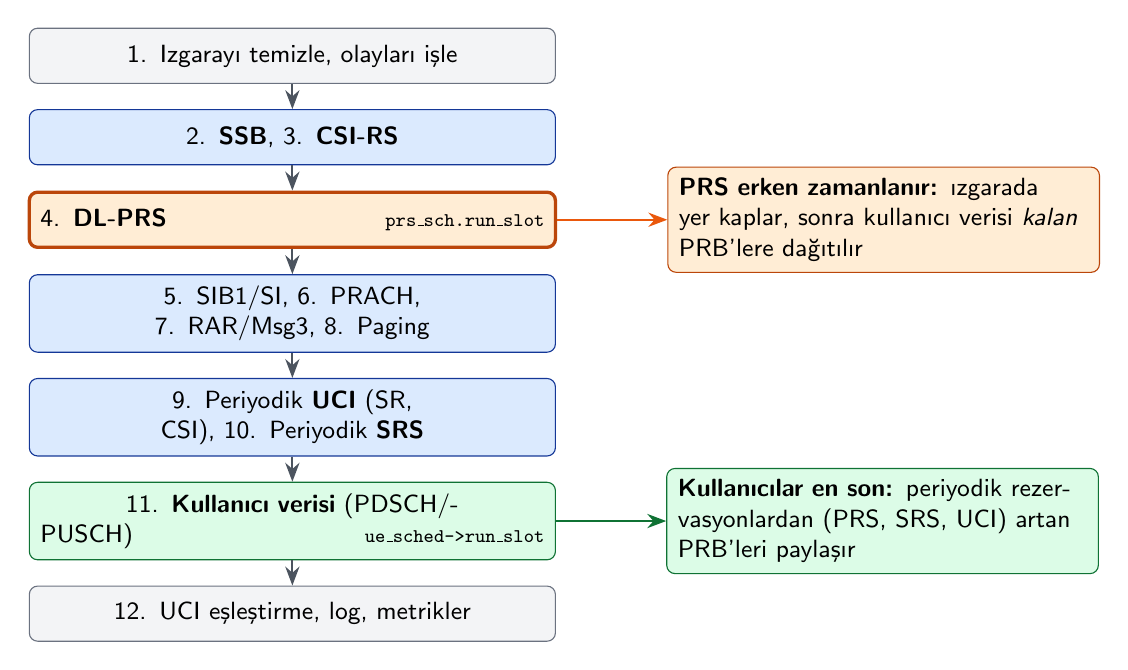
\begin{tikzpicture}[node distance=3.2mm,every node/.style={font=\sffamily\small}]
  \node[ndn,text width=6.4cm] (a) {1. Izgarayı temizle, olayları işle};
  \node[nd,text width=6.4cm,below=of a] (b) {2. \textbf{SSB}, 3. \textbf{CSI-RS}};
  \node[ndw,text width=6.4cm,below=of b,line width=1.2pt] (c) {4. \textbf{DL-PRS} \hfill{\scriptsize \texttt{prs\_sch.run\_slot}}};
  \node[nd,text width=6.4cm,below=of c] (d) {5. SIB1/SI, 6. PRACH, 7. RAR/Msg3, 8. Paging};
  \node[nd,text width=6.4cm,below=of d] (e) {9. Periyodik \textbf{UCI} (SR, CSI), 10. Periyodik \textbf{SRS}};
  \node[ndg,text width=6.4cm,below=of e] (f) {11. \textbf{Kullanıcı verisi} (PDSCH/PUSCH) \hfill{\scriptsize \texttt{ue\_sched->run\_slot}}};
  \node[ndn,text width=6.4cm,below=of f] (g) {12. UCI eşleştirme, log, metrikler};
  \foreach \x/\y in {a/b,b/c,c/d,d/e,e/f,f/g} \draw[ar] (\x) -- (\y);
  \node[ndw,text width=5.2cm,right=14mm of c,align=left] (note1) {\textbf{PRS erken zamanlanır:} ızgarada yer kaplar, sonra kullanıcı verisi \emph{kalan} PRB'lere dağıtılır};
  \draw[ar,color=warn] (c.east) -- (note1.west);
  \node[ndg,text width=5.2cm,right=14mm of f,align=left] (note2) {\textbf{Kullanıcılar en son:} periyodik rezervasyonlardan (PRS, SRS, UCI) artan PRB'leri paylaşır};
  \draw[ar,color=good!70!black] (f.east) -- (note2.west);
\end{tikzpicture}
\caption{OCUDU scheduler'ının slot başına işlem sırası (\texttt{cell\_scheduler.cpp}). Turuncu adım: \textbf{sensing sinyali olarak kullanabileceğimiz PRS}.}
\label{fig:slotflow}
\end{figure}

\textbf{Anahtar fikir:} \emph{periyodik, önceden bilinen} sinyaller (SSB, CSI-RS, \textbf{PRS}, PRACH, UCI, SRS) önce ızgarada yerini alır; kullanıcı verisi \emph{kalan kaynağı} alır.
Dokümandaki ifadeyle: ``\textit{uci\_scheduler ve srs\_scheduler, UE tahsisinden önce periyodik fırsatlarını rezerve etmek zorunda olduğu için UE zamanlamadan önce çalışır}''.
Sensing'in kaynak ihtiyacı da tam bu türdendir: periyodik ve önceden bilinen.

\subsection{Büyük bulgu: OCUDU'da PRS zaten var}\label{sec:prs}

Sensing için ihtiyaç duyduğumuz \emph{gönderici tarafının} büyük bölümü OCUDU'da hazır:

\begingroup\sffamily\small
\begin{xltabular}{\textwidth}{@{}p{4.9cm}X@{}}
\toprule
\textbf{Dosya} & \textbf{Ne yapıyor?} \\
\midrule
\kod{lib/scheduler/common_scheduling/prs_scheduler.cpp} & \textbf{MAC'te DL-PRS zamanlayıcısı.} PRS kaynak kümelerini periyoda, ofsete, tekrar faktörüne, \emph{muting} desenlerine göre slotlara yerleştirir. \\
\kod{lib/phy/upper/signal_processors/prs/prs_generator_impl.cpp} & \textbf{PHY'de PRS dizisini üretir} (standarttaki dizi, TS 38.211 \S7.4.1.7). \\
\kod{lib/fapi_adaptor/mac/p7/pdu_translators/prs.cpp} ve \kod{.../phy/p7/.../prs.cpp} & MAC'in PRS isteğini PHY'nin anlayacağı biçime çevirir. \\
\kod{lib/f1ap/cu_cp/procedures/f1ap_positioning_*.cpp} & CU--DU arasında konumlandırma prosedürleri. \\
\kod{lib/nrppa/}, \kod{lib/lpp/} & Konumlandırma protokolleri. \\
\bottomrule
\end{xltabular}
\endgroup

PRS'in kapladığı kaynağı rezerve eden asıl satır (\texttt{prs\_scheduler.cpp}, \texttt{schedule\_slot}):

\begin{lstlisting}
slot_alloc.dl_res_grid.fill(grant_info{pdu.scs, pdu.symbols, pdu.crbs});
\end{lstlisting}

Yani PRS'in kapladığı \emph{sembol aralığı} ($\times$ PRB aralığı), ızgarada ``dolu'' olarak işaretlenir. Kullanıcı verisi scheduler'ı bu bölgeye tahsis yapamaz.

\subsubsection{PRS yapılandırması (YAML)}

PRS, hücre yapılandırmasında \texttt{cell\_cfg:} altında \texttt{prs:} bölümüyle açılır. Bu yapılandırmayı denedik; gNB hücreyi açtı. Örnek (PRS her 4 slotta bir, 20\,MHz hücre, 104 PRB):

\begin{lstlisting}
cell_cfg:
  dl_arfcn: 368500
  band: 3
  channel_bandwidth_MHz: 20
  common_scs: 15
  prs:
    resource_sets:
      - comb_size: 2
        periodicity_slots: 4
        slot_offset: 1
        nof_symbols: 12
        bandwidth_prbs: 104
        resources:
          - sequence_id: 1
            re_offset: 0
            slot_offset: 0
            symbol_offset: 2
\end{lstlisting}

\begingroup\sffamily\small
\begin{xltabular}{\textwidth}{@{}p{3.4cm}p{4.6cm}X@{}}
\toprule
\textbf{Parametre} & \textbf{Anlamı} & \textbf{Geçerli değerler} \\
\midrule
\texttt{periodicity\_slots} & PRS kaç slotta bir tekrarlanır ($T_{PRS}$) & 4, 5, 8, 10, 16, 20, 32, 40, 64, 80, 160, \ldots \\
\texttt{slot\_offset} & Periyot içindeki başlangıç slotu & $0 \ldots T-1$ \\
\texttt{nof\_symbols} & Her kaynağın OFDM sembol sayısı & 2, 4, 6, 12 \\
\texttt{bandwidth\_prbs} & PRS'in kapladığı PRB (4'ün katı) & 24 \ldots 272 \\
\texttt{comb\_size} & Comb (alt taşıyıcı seyreltme) & 2, 4, 6, 12 \\
\texttt{repetition\_factor}, \texttt{time\_gap} & Tekrar sayısı ve aralığı & 1--32 \\
\texttt{power\_offset\_db} & Güç ofseti & $-60 \ldots 50$ \\
\bottomrule
\end{xltabular}
\endgroup

\begin{dikkat}[OCUDU yapılandırmayı doğrular]
\texttt{slot\_offset: 0} ve periyot 10 verdiğimizde gNB \emph{başlamadı}:
\texttt{Detected a collision between the SSB occasion (ssb-Index=0) and the DL-PRS resource ... in slot 0 (period 10 slots)}.
PRS, SSB ile çakışamaz; \texttt{slot\_offset: 1} ile çözüldü. Ayrıca PDSCH için \texttt{mcs\_table: qam64} verilmezse
``256QAM MCS table cannot be used for PDSCH with fallback DCI format'' hatası alınır. Bunlar \emph{doğrulama} mesajlarıdır, hata değil.
\end{dikkat}

\subsubsection{Ölçüm: PRS yükü arttıkça DL throughput ne kadar düşer?}

OCUDU'yu radyosuz modda (\texttt{testmode}, \texttt{ru\_dummy}, 20\,MHz FDD, 15\,kHz SCS, 1 sanal UE, tam tamponlu indirme trafiği) çalıştırıp PRS periyodunu değiştirdik.
Her koşu yaklaşık 30\,s, tablodaki değerler son 15 satırın ortalamasıdır:

\begin{figure}[H]
\centering
\includegraphics[width=0.82\textwidth]{sekiller/fig_ocudu_prs.pdf}
\caption{\textbf{Gerçek OCUDU ölçümü} (WSL2, testmode). Mavi: tüm banda PRS (104/106 PRB). Kesikli çizgi: kuram $59\,(1-1/T_{PRS})$.
Turuncu: $T=4$ ama PRS yalnızca 52 PRB'de. Veri: \texttt{ogretici/veri/ocudu\_prs\_sweep.csv}.}
\label{fig:ocudu-prs}
\end{figure}

\begin{center}
\sffamily\small
\begin{tabular}{@{}lrrrrr@{}}
\toprule
\textbf{Koşul} & $T_{PRS}$ & sembol & PRB & \textbf{DL (Mbps)} & başarılı blok/s \\
\midrule
Sensing yok & -- & -- & -- & 59,0 & 1000 \\
$T=80$ & 80 & 12 & 104 & 58,0 & 987 \\
$T=40$ & 40 & 12 & 104 & 57,8 & 972 \\
$T=20$ & 20 & 12 & 104 & 56,0 & 950 \\
$T=10$ & 10 & 12 & 104 & 53,0 & 900 \\
$T=8$ & 8 & 12 & 104 & 50,9 & 874 \\
$T=4$ & 4 & 12 & 104 & 43,8 & 749 \\
$T=4$, yarım bant & 4 & 12 & 52 & 51,0 & 1000 \\
$T=4$, 4 sembol & 4 & 4 & 104 & 43,8 & 748 \\
\bottomrule
\end{tabular}
\end{center}
{\sffamily\footnotesize\color{muted} UL throughput tüm koşullarda $\approx$77,2\,Mbps, yani PRS'ten etkilenmedi (PRS DL sinyalidir).}

\begin{bulgu}[Dört gözlem ve açık soru]
\textbf{(1) H1 ile uyumlu.} Tüm banda PRS koyunca DL throughput, PRS'li slot oranı kadar düşüyor: $T=4$ (\%25 slot) $\Rightarrow$ 59,0 $\rightarrow$ 43,8\,Mbps (\%26 azalma). 1000 slotluk saniyede 749 başarılı blok.\\
\textbf{(2) Bant payı önemli.} PRS'i bandın yarısına (52 PRB) koyunca, aynı periyotta \emph{slot kaybı olmadı} (1000 blok) ve düşüş yalnızca 59,0 $\rightarrow$ 51,0\,Mbps (\%13,6): yaklaşık $0{,}25\times\frac{52}{106}=\%12{,}3$. Scheduler, PRS'in kaplamadığı PRB'lere veri tahsis etmeye devam ediyor.\\
\textbf{(3) UL etkilenmiyor.} PRS bir DL sinyali olduğu için UL değişmedi.\\
\textbf{(4) Açık soru: sembol sayısı neden etkisiz?} 12 sembollük PRS ile 4 sembollük PRS \emph{aynı} kaybı verdi (43,8\,Mbps). Kuramda 4 sembol daha az kaynak kaplamalı. Olası açıklama:
PDSCH tahsisinin zaman ekseni sabit bir sembol aralığına yayılıyor ve PRS ile çakışan PRB'ler o slotta tümden kullanılamıyor. Bu \textbf{doğrulanmadı}, OCUDU'daki PDSCH tahsis koduna (\kod{lib/scheduler/ue_scheduling/}) bakılarak cevaplanmalı.
Cevap, ``sensing kaynak payı'' tanımımızı doğrudan etkiler (TR~38.765'teki Tip~3 kaynak!).
\end{bulgu}

\begin{dikkat}[Bu ölçümün sınırları]
\textbf{(i)} Her koşul \emph{tek koşu}, 15 saniyelik ortalama; tekrarlayıp hata çubuğu eklemek gerekir. (Betikleri taşıdıktan sonra $T=20$ koşusunu bir kez daha çalıştırdık ve \emph{aynı} değerleri aldık: 56\,Mbps, 950 blok/s. Yani bu ortamda koşular arası oynaklık küçük görünüyor, ama bunu 5 koşuyla kanıtlamak gerekir.) \textbf{(ii)} WSL2 gerçek zamanlı değil; log'da \texttt{Real-time failure in RU: received late DL request} uyarıları vardı.
\textbf{(iii)} \texttt{testmode} gerçek radyo, gerçek kanal ve gerçek UE içermez: yalnızca MAC/PHY'yi uyarır. Sayıların \emph{mutlak değeri} (59\,Mbps) gerçek bir sistem için geçerli değildir; \emph{eğilim} geçerlidir.
\textbf{(iv)} Bu deney sensing'i değil, yalnızca \emph{PRS'in kaynak maliyetini} ölçer. Alıcı tarafı (yankıyı işleyen) yoktur.
\end{dikkat}

\subsection{Slicing: PRB oranıyla kaynak ayırma}\label{sec:slicing}

OCUDU'da kullanıcı trafiği \emph{dilimlenebilir} (network slicing). Her dilim için yapılandırmada (\texttt{du\_high\_config.h}, \texttt{du\_high\_unit\_cell\_slice\_sched\_config}):
\begin{itemize}
\item \texttt{min\_prb\_policy\_ratio}: dilime garanti edilen en az PRB yüzdesi,
\item \texttt{max\_prb\_policy\_ratio}: en çok PRB yüzdesi,
\item \texttt{ded\_prb\_policy\_ratio}: dilime \emph{ayrılmış} (dedicated) PRB yüzdesi,
\item \texttt{priority}: dilim önceliği.
\end{itemize}
Ayrıca çalışma anında dilim oranı \texttt{rrm\_policy\_ratio\_set} uzaktan komutuyla değiştirilebilir. Scheduler'ın içinde \texttt{inter\_slice\_scheduler} dilimleri sıralar, \texttt{intra\_slice\_scheduler} dilimin içinde dağıtır.
Scheduler politikaları: \texttt{time\_rr} (round-robin) ve \texttt{time\_qos} (QoS-farkında, PF katsayısı yapılandırılabilir).

\textbf{Fikir (denenmedi):} ``sensing'' için bir dilim tanımlayıp \texttt{ded\_prb\_policy\_ratio} ile kaynak ayırmak, PRS'e alternatif ve \emph{koda dokunmadan} bir sensing-yükü emülasyonu olabilir.
Bunun gerçekten iş görüp görmediği bir pilot görevdir (Bölüm~\ref{sec:pilot}).

\subsection{Nereye ekleme yapabiliriz?}\label{sec:ekleme}

Gerçek bir kod tabanına ekleme yaparken \textbf{en az değişiklikle başlayıp gerekirse artırmak} esastır. Dört seviye:

\begingroup\sffamily\small
\begin{xltabular}{\textwidth}{@{}p{0.5cm}p{2.9cm}p{3.6cm}Xp{1.5cm}@{}}
\toprule
 & \textbf{Seviye} & \textbf{Ne yapılır} & \textbf{Ne öğrenir/elde ederiz} & \textbf{Emek} \\
\midrule
A & \textbf{Yapılandırma (kod yok)} & \texttt{prs:} bölümünü ve dilimleri YAML'da ayarlayıp \texttt{testmode} ile ölç & PRS yükünün haberleşmeye maliyeti (\textbf{yaptık}, Şekil~\ref{fig:ocudu-prs}) & \textcolor{good}{düşük} \\
B & \textbf{Ölçüm/log ekleme} & Scheduler metriklerinden PRS'li slot oranı, kaybolan PRB, Tip~1/2/3 kaynakları çıkarmak & TR~38.765'in ``sensing kaynak oranı'' metriğini \emph{gerçek kodda} hesaplamak & \textcolor{good}{düşük--orta} \\
C & \textbf{Politika ekleme} & Yüke göre PRS periyodunu/bandını uyarlayan basit bir kural ($\alpha$ yük arttıkça küçülür) & H3: \emph{uyarlanır} politikanın sabitten iyi olup olmadığı & \textcolor{warn}{orta--yüksek} \\
D & \textbf{Alıcı tarafı sensing} & Yankı işleme (range-Doppler), SenF/NsAP arayüzü & Tam ISAC. OCUDU'da yok; bizim kapsamımız dışı & \textcolor{bad}{çok yüksek} \\
\bottomrule
\end{xltabular}
\endgroup

\textbf{Önerimiz:} \textbf{A} ve \textbf{B}'yi hedefleyin; \textbf{C}'yi ``zaman kalırsa'' bırakın; \textbf{D}'yi yalnızca \emph{tasarım diyagramı} olarak (bkz.\ Bölüm~\ref{sec:senf}) yapın.
Bunun nedeni basit: ana sorumuz haberleşme tarafına etkiyi ölçmek, A--B bunu zaten verir.

\subsubsection{Kod geliştirme döngüsü (A ve B için)}

\begin{lstlisting}
# 1) Kodu degistir (Windows'ta VS Code ile, Remote-WSL uzerinden)
cd ~/ehb415/ocudu && code .

# 2) Sadece gnb'yi yeniden derle (degisen dosyalar icin hizli, ccache sayesinde)
cd ~/ehb415/ocudu/build && make -j4 gnb

# 3) Calistir (yapilandirma dosyalarini birlestirebilirsin: -c a.yml -c b.yml)
./apps/gnb/gnb -c /mnt/c/Users/<kullanici>/Desktop/EHB415/kurulum/ocudu_testmode.yml
# gNB acildiktan sonra konsola "t" yazip Enter: metrik tablosu gorunur (bu makinede boyle gozlendi)
\end{lstlisting}

\begin{dikkat}[Gerçek bir geliştirici gibi çalış]
Her değişiklikten sonra \texttt{git diff} ile ne değiştiğine bak ve \emph{küçük adımlarla} ilerle: bir ölçüm satırı ekle, derle, çalıştır, sonucu gör. Büyük değişiklikleri tek seferde yapmak,
OCUDU gibi yüz binlerce satırlık bir kod tabanında hatayı bulmayı imkânsız hale getirir. Ayrıca kendi değişikliklerini \emph{yama (patch) dosyası} olarak saklayın; OCUDU deposunun kendisini projemizin reposuna kopyalamıyoruz.
\end{dikkat}

\section{Pilot görevler ve görev dağılımı}\label{sec:pilot}

\subsection{Pilot hafta: herkes aynı üç mini deneyi yapar}

\textbf{Amaç:} Herkes, uzmanlaşmadan \emph{önce}, üç aracın her birinde bir sonuç üretsin. Böylece ``OCUDU'cu'' ns-3'ün ne yaptığını, ``Sionna'cı'' scheduler'ın etkisini görmüş olur
ve toplantılarda aynı dili konuşuruz. Her pilot yarım gün sürer. Kurulumlar \texttt{kurulum/} klasöründeki dokümanlarla yapılmış olmalı.

\begingroup\sffamily\small
\begin{xltabular}{\textwidth}{@{}p{2cm}p{3.6cm}Xp{2.6cm}@{}}
\toprule
\textbf{Pilot} & \textbf{Araç} & \textbf{Ne yapılır} & \textbf{Çıktı} \\
\midrule
Pilot-1 & OCUDU & PRS yükünü değiştirip DL throughput'u ölç & Tablo + 1 paragraf \\
Pilot-2 & ns-3 / 5G-LENA & UE sayısına göre throughput ve gecikmeyi ölç & Tablo + 1 grafik \\
Pilot-3 & Sionna (radar) & Range-Doppler haritası, çözünürlük ve boşluk deneyi & 1 grafik + 1 paragraf \\
\bottomrule
\end{xltabular}
\endgroup

Her pilotun sonunda bir \textbf{soru kartı} var: kendi cümlelerinizle cevaplayın (her biri 2--3 cümle). Ek~\ref{ek:cevap}'te \emph{beklenen cevaplar} yönetici için verilmiştir;
cevapları yazmadan önce bakmayın, öğrenmenin yolu o.

\subsubsection{Pilot-1: OCUDU'da PRS maliyetini ölç}

\begin{pilot}[Pilot-1: adımlar]
\begin{enumerate}[leftmargin=1.5em]
\item Ubuntu'da: \texttt{cd \textasciitilde/ehb415/ocudu/build/apps/gnb}
\item Temel koşu (PRS yok): \texttt{./gnb -c /mnt/c/Users/<kullanici>/Desktop/EHB415/kurulum/ocudu\_testmode.yml}. gNB açılınca \texttt{t} yazıp Enter; tablo gelir. DL \texttt{brate} sütununu not et (59\,M civarı). \texttt{Ctrl+C} ile kapat.
\item Bir kopya yapılandırma dosyası hazırla, \texttt{cell\_cfg:} altına \texttt{pdsch:}'den önce Bölüm~\ref{sec:prs}'deki \texttt{prs:} bloğunu ekle. Hazır örnek: \texttt{ogretici/veri/ocudu\_p4\_config.yml} ($T=4$).
\item Aynı şekilde çalıştır; \texttt{brate} ve \texttt{ok} sütunlarını not et. $T$ değerini 8, 20, 40 yap, her seferinde tekrarla.
\item \texttt{bandwidth\_prbs: 52} ile $T=4$'ü dene.
\end{enumerate}
\textbf{Kısayol:} adım 3--5'i otomatikleştiren betik: \texttt{bash ogretici/betikler/ocudu\_prs\_kos.sh p4 4 12 104} (etiket, periyot, sembol, PRB). Önce elle yapın, sonra betiği kullanın.
\textbf{Çıktı:} $T$ ve \texttt{bandwidth\_prbs}'e göre DL throughput tablosu. Bölüm~\ref{sec:prs}'deki tabloyla karşılaştır.
\end{pilot}

\begin{ipucu}[Soru kartı: Pilot-1]
\textbf{(1)} PRS her 4 slotta bir olunca DL throughput neden yaklaşık \%25 düştü? \quad
\textbf{(2)} PRS'i bandın yarısına koyunca neden yalnızca yaklaşık \%13 düştü? \quad
\textbf{(3)} Bu deney TR 38.765'teki Tip~1, 2 ve 3 kaynakların hangisine karşılık gelir?
\end{ipucu}

\subsubsection{Pilot-2: ns-3'te UE sayısını artır}

\begin{pilot}[Pilot-2: adımlar]
\begin{enumerate}[leftmargin=1.5em]
\item Ubuntu'da: \texttt{cd \textasciitilde/ehb415/ns-3-dev}
\item \texttt{./ns3 run "cttc-nr-demo --ueNumPergNb=1"}, sonra 2, 5, 10, 20 için tekrarla.
\item Her koşuda çıktıdaki akış sayısını, her akışın \texttt{Throughput} ve \texttt{Mean delay} değerini ve son satırdaki \texttt{Mean flow throughput}/\texttt{Mean flow delay}'i not et.
\item Toplam throughput'u (akışların toplamı) ve ortalama gecikmeyi UE sayısına karşı tabloya yaz; Excel veya Python ile grafiğe çevir.
\end{enumerate}
\textbf{Çıktı:} Bölüm~\ref{sec:ns3}'teki gibi bir tablo ve grafik.
\end{pilot}

\begin{ipucu}[Soru kartı: Pilot-2]
\textbf{(1)} Gecikme neden 0,28\,ms'den yaklaşık 124\,ms'ye çıktı? \quad
\textbf{(2)} Toplam throughput neden UE sayısıyla doğrusal artmadı? \quad
\textbf{(3)} Sensing yükünü bu senaryoya koymak için Bölüm~\ref{sec:ns3tasarim}'deki (a), (b), (c) yollarından hangisini önerirsin, neden?
\end{ipucu}

\subsubsection{Pilot-3: Radar ve boşluk deneyi}

\begin{pilot}[Pilot-3: adımlar]
\begin{enumerate}[leftmargin=1.5em]
\item Windows PowerShell'de: \texttt{C:\textbackslash Users\textbackslash <kullanici>\textbackslash venvs\textbackslash ehb415\textbackslash Scripts\textbackslash python.exe kurulum\textbackslash sionna\_dogrulama.py}. Çıktıdaki gerçek ve tahmin edilen menzil/hızı not et.
\item \texttt{ogretici\textbackslash betikler\textbackslash make\_figs.py} içindeki \texttt{fig\_gap()} fonksiyonunu çalıştır (\texttt{pip install pandas matplotlib} gerekebilir).
\item Betikte hedef mesafesini ve hızını değiştir, haritada tepenin de kaydığını gör.
\item Sembol sayısını $M=128$'den 32'ye düşür; çözünürlüğün nasıl değiştiğini formülle karşılaştır.
\end{enumerate}
\textbf{Çıktı:} Bölüm~\ref{sec:sionna}'deki gibi bir grafik ve ``neden?'' paragrafı.
\end{pilot}

\begin{ipucu}[Soru kartı: Pilot-3]
\textbf{(1)} $M=128$ yerine 32 sembol kullanınca hız çözünürlüğü kaç kat değişir? \quad
\textbf{(2)} Boşluklar neden yan lobları yükseltir? \quad
\textbf{(3)} Haberleşme scheduler'ı sensing için \emph{neyi garanti etmeli}?
\end{ipucu}

\subsection{Dört kişilik görev dağılımı}\label{sec:roller}

Pilotlardan sonra herkes bir \textbf{rol} üstlenir. Her rolün somut bir ``Faz-1 çıktısı'' var (çıktısı olmayan görev vermiyoruz). Dördüncü rol, proje yöneticisinin entegrasyon ve standart işi.

\begingroup\sffamily\small
\begin{xltabular}{\textwidth}{@{}p{1.1cm}p{2.7cm}Xp{3.4cm}@{}}
\toprule
\textbf{Rol} & \textbf{Alan} & \textbf{Faz-1 çıktıları (somut)} & \textbf{Önce okuma} \\
\midrule
R1 & \textbf{Standart, metrik, entegrasyon} &
  (a) \texttt{docs/metrics.md}: TR~38.765 \S4.1 ve \S6.2'den metrik sözlüğü (formüllerle). (b) Dickerson modelini ($\alpha$, $T(\eta)$) bir tabloya/betiğe dök. (c) Üç aracın sonuçlarını \emph{aynı $\alpha$ eksenine} getiren ortak grafik şablonu. &
  TR 38.765 \S4, 6.2, 9; Lin \cite{lin}; Dickerson \cite{dickerson} \\
R2 & \textbf{Sionna} &
  (a) Sensing performansı eğrisi: bant ($W$) ve sembol sayısına ($M$) göre menzil/hız hatası ve tespit olasılığı. (b) Boşluk deneyini gerçekçileştir (SNR, çok hedef). (c) Sionna RT öğreticilerinden 3'ünü çalıştır. &
  Wei \cite{wei}, Khosroshahi \cite{khos}, NIST \cite{nist}; Sionna RT \cite{sionnart} \\
R3 & \textbf{ns-3 / 5G-LENA} &
  (a) Sensing yükünü (a) ve (b) yollarıyla ekle (Bölüm~\ref{sec:ns3tasarim}). (b) $\alpha$'ya göre throughput/gecikme/PLR taraması, CSV + grafik. (c) 5G-LENA scheduler sınıflarının tablosu. &
  SioLENA \cite{siolena}; Koutlia \cite{koutlia}; Capozzi \cite{capozzi} \\
R4 & \textbf{OCUDU} &
  (a) Bölüm~\ref{sec:prs}'deki ölçümü \emph{tekrarla ve hata çubuğu ekle} (örn.\ 5 koşu). (b) ``Sembol sayısı neden etkisiz?'' sorusunu kodu okuyarak cevapla. (c) Slicing ile (\texttt{ded\_prb\_policy\_ratio}) sensing emülasyonunu dene. (d) Kod haritası ve ``sensing nereye takılır'' diyagramı. &
  Lindenschmitt \cite{linden}; Gurung \cite{gurung}; OCUDU \texttt{lib/scheduler/README.md} \\
\bottomrule
\end{xltabular}
\endgroup

\textbf{Ortak çalışma (``ikinci göz''):} her çıktı bir başkası tarafından \emph{yeniden üretilmeden} ``bitti'' sayılmaz.
Öneri eşleşmeleri: R2 $\leftrightarrow$ R3 (kanal/ağ köprüsü, SioLENA), R3 $\leftrightarrow$ R4 (ns-3 sonuçlarıyla OCUDU ölçümünü karşılaştırma), R1 $\leftrightarrow$ herkes (metrik tutarlılığı).

\begin{dikkat}[Rolleri neden böyle böldük?]
Üç araç birbirinden \emph{bağımsız} çalışabilir, ama sonuçları \textbf{aynı eksende} buluşmalı. Bunu garanti eden rol R1'dir: herkes sonucunu $\alpha$ cinsinden ve R1'in metrik sözlüğündeki tanımlarla raporlar.
Aksi halde üç farklı ``overhead'' tanımıyla üç uyumsuz grafik çıkar.
\end{dikkat}

\subsection{Hedef grafik: hepimizin üzerinde çalıştığı tek şekil}

Projenin ``kahramanı'' şekil şu şemadaki gibi olacak (\textbf{bu bir şematiktir, veri değildir}):

\begin{figure}[H]
\centering
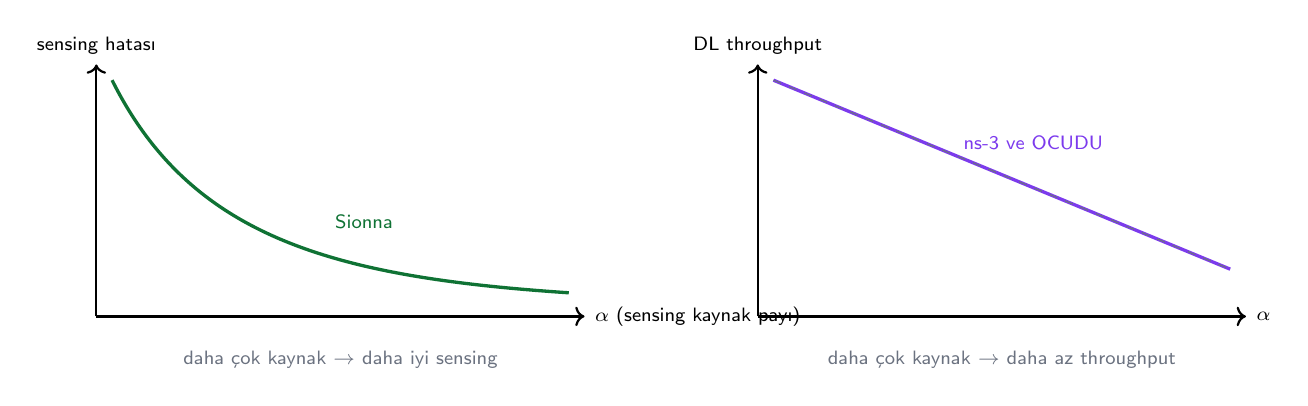
\begin{tikzpicture}[x=1cm,y=1cm]
  \begin{scope}[shift={(0,0)}]
    \draw[->,thick] (0,0) -- (6.2,0) node[right,font=\sffamily\scriptsize] {$\alpha$ (sensing kaynak payı)};
    \draw[->,thick] (0,0) -- (0,3.2) node[above,font=\sffamily\scriptsize] {sensing hatası};
    \draw[very thick,good!70!black] (0.2,3.0) .. controls (1.2,1.0) and (3,0.5) .. (6,0.3);
    \node[font=\sffamily\scriptsize,color=good!70!black] at (3.4,1.2) {Sionna};
    \node[font=\sffamily\scriptsize,color=muted] at (3.1,-0.55) {daha çok kaynak $\rightarrow$ daha iyi sensing};
  \end{scope}
  \begin{scope}[shift={(8.4,0)}]
    \draw[->,thick] (0,0) -- (6.2,0) node[right,font=\sffamily\scriptsize] {$\alpha$};
    \draw[->,thick] (0,0) -- (0,3.2) node[above,font=\sffamily\scriptsize] {DL throughput};
    \draw[very thick,purp] (0.2,3.0) -- (6,0.6);
    \node[font=\sffamily\scriptsize,color=purp] at (3.5,2.2) {ns-3 ve OCUDU};
    \draw[dashed,color=muted] (0.2,3.0) -- (6,0.6);
    \node[font=\sffamily\scriptsize,color=muted] at (3.1,-0.55) {daha çok kaynak $\rightarrow$ daha az throughput};
  \end{scope}
\end{tikzpicture}
\caption{\textbf{Şematik} (veri değil): iki ters eğri aynı $\alpha$ ekseninde. Proje, bu iki eğrinin gerçek hâlini üretmek ve ``çalışma noktası'' (hem sensing yeterli hem haberleşme kabul edilebilir) bölgesini bulmaktır.}
\end{figure}

\subsection{Haftalık plan önerisi}

Kesin teslim tarihlerini bilmediğimden aşağıdaki \textbf{12 haftalık bir öneridir}; ara rapor/final tarihine göre ölçeklenmelidir.

\begingroup\sffamily\small
\begin{xltabular}{\textwidth}{@{}p{1.3cm}X@{}}
\toprule
\textbf{Hafta} & \textbf{Hedef} \\
\midrule
1 & Kurulumlar bitti. \textbf{Pilot-1, 2, 3} (herkes). Soru kartları cevaplandı. \\
2 & Okuma: herkes Bölüm~\ref{sec:buyuk}--\ref{sec:3gpp} + kendi rolünün makaleleri. \textbf{Karar toplantısı:} sensing yükünü nasıl temsil ediyoruz (Bölüm~\ref{sec:ns3tasarim} a/b/c), hangi metrikler. \\
3--4 & Rol çıktıları (Faz-1). Haftalık 30 dakikalık ``gördüğümü anlat'' toplantısı. \\
5 & \textbf{İlk entegrasyon:} üç aracın sonucu aynı $\alpha$ ekseninde, taslak ortak grafik. \\
6 & \textbf{Ara rapor.} Boşluklar ve riskler listelenir. \\
7--9 & Genişletme: OCUDU seviye~B (metrik/log), Sionna RT ile gerçekçi kanal, ns-3'te (c) yolu veya SioLENA (zaman kalırsa). \\
10 & Tekrar koşular, hata çubukları, sınırlılıklar bölümü. \\
11 & Rapor yazımı. \\
12 & Gözden geçirme, tekrar üretilebilirlik kontrolü (başkası komutlarla aynı sonucu alıyor mu?), teslim. \\
\bottomrule
\end{xltabular}
\endgroup

\subsection{Riskler ve nasıl yönetiriz}

\begingroup\sffamily\small
\begin{xltabular}{\textwidth}{@{}p{4.4cm}Xp{3.6cm}@{}}
\toprule
\textbf{Risk} & \textbf{Etkisi} & \textbf{Önlem} \\
\midrule
Ölçümler tek koşu, WSL2 gerçek zamanlı değil & Sayılar oynak olabilir & R4: 5 koşu + hata çubuğu \\
``Sembol sayısı etkisiz'' bulgusunun nedeni belirsiz & Tip~3 kaynak tanımımız yanlış olabilir & R4: PDSCH tahsis kodunu oku (Bölüm~\ref{sec:prs}) \\
5G-LENA'da sensing modeli yok & Deney tasarımı belirsiz & Karar toplantısı (hafta 2), (a)/(b) yolu \\
SioLENA ayrı ns-3 ağacı, eski Sionna & Entegrasyon zor & İkinci aşama; ana sonuca bağımlı yapma \\
Rapor yazılmadan zaman biter & Teslim riski & Hafta 5'te taslak grafik, hafta 11 yazım \\
\bottomrule
\end{xltabular}
\endgroup

\section{Makale okuma rehberi}\label{sec:okuma}

\subsection{Google Scholar'a ne yazmalı?}

Scholar, arama kutusundaki \textbf{tırnak içindeki ifadeleri aynen} arar ve çok kelimeli sorgularda çok geniş sonuç döndürür. Bu yüzden
\emph{tırnaklı anahtar ifadeler} ve yanlarında 1--2 serbest kelime kullanın. Aşağıdaki sorgular, bu projenin her alt konusunu kapsayacak şekilde tasarlandı.
\textbf{Sorgulardaki sonuçları ben kontrol etmedim}; sonuç sayısı ve sırası değişir. Bulduklarınızı Bölüm~\ref{sec:okuma-liste}'teki listeyle karşılaştırın.

\begingroup\sffamily\small
\begin{xltabular}{\textwidth}{@{}p{0.5cm}p{7.0cm}X@{}}
\toprule
 & \textbf{Sorgu (kopyala-yapıştır)} & \textbf{Ne ararsın / ne işine yarar} \\
\midrule
1 & \texttt{"integrated sensing and communication" "5G NR" "positioning reference signal"} & PRS ile sensing yapan çalışmalar; sinyal tasarımı ve sonuçlar. \\
2 & \texttt{"ISAC" "resource allocation" "5G NR" "sensing overhead"} & \textbf{Ana sorumuz:} sensing kaynak payı ve throughput kaybı. \\
3 & \texttt{"ISAC" "3GPP" "Release 19" OR "Release 20" sensing "channel model"} & Standart durumu, kanal modeli. \\
4 & \texttt{"gNB" "monostatic sensing" UAV detection "5G NR"} & TR~38.765'in senaryosuyla aynı çalışmalar. \\
5 & \texttt{"ISAC" "O-RAN" OR "OpenRAN" xApp sensing srsRAN OR OpenAirInterface} & Açık RAN'a sensing entegrasyon mimarileri (OCUDU tarafı). \\
6 & \texttt{"Sionna" "ray tracing" sensing OR radar OFDM} & Sionna ile sensing/ISAC uygulamaları, hazır kod. \\
7 & \texttt{"ns-3" "5G-LENA" sensing OR ISAC} & ns-3'te sensing modelleme (az çıkması beklenir; boşluğu gösterir). \\
8 & \texttt{"OFDM radar" "range-Doppler" "mobile network" tutorial} & Radyo sinyal işleme temelleri, öğretici nitelikli. \\
9 & \texttt{"self-interference" "monostatic" "base station" sensing isolation} & Öz-girişim, neden zor, hangi izolasyon yeter. \\
10 & \texttt{"ghost targets" PRS comb sensing} & PRS tabanlı sensing'in bilinen sorunu ve çözümleri. \\
11 & \texttt{"communication-sensing tradeoff" OR "sensing-communication tradeoff" ISAC "Cramer-Rao"} & Teorik ödünleşim (R1 için, matematik yoğun). \\
12 & \texttt{"sensing-assisted" scheduling OR "beam management" 5G ISAC} & Tersine yön: sensing'in haberleşmeye \emph{katkısı} (rapora zenginlik). \\
\bottomrule
\end{xltabular}
\endgroup

\subsubsection{Scholar'ı verimli kullanmak}

\begin{itemize}
\item Soldaki menüden \textbf{``Since 2024''} (veya ``Since 2025'') seçin: alan hızlı değişiyor, 2022 öncesi çalışmalar çoğu zaman eski.
\item \textbf{``Cited by''} bağlantısı: bir makaleyi \emph{atıf yapan yeni makaleler} üzerinden ileriye doğru izleyin (en değerli ipucu).
\item \textbf{``Related articles''} ve \textbf{``Versions''}: arXiv sürümünü bulun, çoğu zaman ücretsizdir.
\item \textbf{``Cite''} $\rightarrow$ BibTeX: rapor kaynakçası için.
\item Bir ``survey'' veya ``tutorial'' bulursanız \emph{önce onu} okuyun: yüzlerce makaleyi sizin için özetler (örn.\ Liu vd.~\cite{liu22}).
\end{itemize}

\subsection{Bir makalede ne aranır? (7 soru)}\label{sec:7soru}

Makaleyi baştan sona okumayın. Önce \textbf{özet, giriş sonu (katkılar) ve sonuç}, sonra şu yedi soruya cevap arayın:

\begin{enumerate}
\item \textbf{Ne ölçüyorlar?} (Hangi metrik: $P_{md}$, hata, throughput?) Bizim metriklerimizle aynı mı?
\item \textbf{Sistem modeli ve parametre tablosu:} bant, SCS, taşıyıcı, anten, hedef. Bizimkiyle karşılaştırılabilir mi?
\item \textbf{Sensing sinyali ne?} (PRS, SRS, DMRS, özel dizi?) Haberleşmeyle nasıl paylaşıyor?
\item \textbf{Kaynak paylaşımı nasıl?} (Zaman, frekans, güç, uzay; sabit mi uyarlanır mı?)
\item \textbf{Hangi araç/simülatör?} (MATLAB, Sionna, ns-3, OAI, srsRAN/OCUDU?) \emph{Kodu paylaşıyorlar mı?}
\item \textbf{Sınırlamalar ve ``future work''} bölümü: bizim için \emph{fırsat} (onların yapmadığı şeyi biz yapıyoruz).
\item \textbf{Bizim projeye tek cümlelik katkısı:} ``X makalesi, Y için Z'yi veriyor.'' Bu cümleyi yazamıyorsanız makaleyi bırakın.
\end{enumerate}

\begin{ipucu}[Her makale için 5 dakikalık not]
Her okuduğunuz makale için ortak bir tabloya \textbf{tek satır} ekleyin: \texttt{Makale | Sinyal | Araç | Kod var mı | Bizim için katkı (1 cümle) | Güven (düşük/orta/yüksek)}.
Dönem sonunda ilgili çalışmalar bölümünün neredeyse hazır olacak.
\end{ipucu}

\subsection{Okuma listesi (indirildi, doğrulandı)}\label{sec:okuma-liste}

Aşağıdaki makaleler \texttt{makaleler/} klasöründe PDF olarak durur; başlık, yazar ve tarihleri arXiv/3GPP'den doğrulandı.
Ayrıntılı ``şurada ne var'' notları \texttt{makaleler/OKUMA\_LISTESI.md} dosyasında.

\begingroup\sffamily\small
\begin{xltabular}{\textwidth}{@{}p{0.9cm}p{4.5cm}p{2.4cm}X@{}}
\toprule
\textbf{Kim} & \textbf{Makale} & \textbf{Önce oku} & \textbf{Neden} \\
\midrule
Herkes & Lin, \emph{ISAC in 3GPP: 5G-Adv.\ to 6G} \cite{lin} & Tamamı (8 s.) & Standart durumunun güncel ve kısa özeti. \\
Herkes & 3GPP TR 38.765 & \S4, 6.2, 9 & Metrikler, kaynak oranı, kararlar. \\
R1, R3 & Dickerson vd.\ \cite{dickerson} & \S III.B, IV.A & Kaynak payı modeli ve throughput formülü. \\
R2 & Khosroshahi vd.\ \cite{khos} & Özet, \S resource allocation & PRS+PDSCH Pareto optimali. \\
R2 & Blandino vd.\ (NIST) \cite{nist} & Özet, sonuçlar & İHA tespiti sonuçları; kod (MATLAB) var. \\
R2 & Wei vd.\ \cite{wei} & CRLB bölümü & Kuramsal sınır; sonuçlarımızı kıyaslamak için. \\
R3 & Ropitault vd.\ (SioLENA) \cite{siolena} & \S III.B, III.C & Sionna RT $\rightarrow$ 5G-LENA kanal köprüsü. \\
R3 & Capozzi vd.\ \cite{capozzi} & \S IV.B--C, V & Scheduler aileleri ve metrik tanımları. \\
R4 & Lindenschmitt vd.\ \cite{linden} & \S 3.3, 4.4, 5 & Sensing işlemenin RAN'daki yeri ve açık sorular. \\
R4 & Gurung vd.\ \cite{gurung} & \S III--IV & OAI + RIC + Sionna RT ile ISAC test düzeneği. \\
İsteğe bağlı & Liu vd.\ \cite{liu22} & \S III, IV.A & Alanın temel tutorial'ı; trade-off teorisi. \\
\bottomrule
\end{xltabular}
\endgroup

\appendix
\section{Sözlük}\label{ek:sozluk}

\begingroup\sffamily\small
\begin{xltabular}{\textwidth}{@{}p{3.2cm}X@{}}
\toprule
\textbf{Terim} & \textbf{Anlamı} \\
\midrule
gNB & 5G baz istasyonu. \\
UE & Kullanıcı cihazı (telefon). \\
NR & 5G'nin radyo arayüzü (New Radio). \\
FR1 & 6\,GHz altı frekans aralığı (bizim senaryolar: 4--4,9\,GHz, band n3 testlerinde 1,8\,GHz). \\
OFDM & Veriyi çok sayıda dar alt taşıyıcıya yayan modülasyon. 5G'nin ve OFDM radarın temeli. \\
SCS & Alt taşıyıcı aralığı (15, 30, 60, 120\,kHz). Slot süresini belirler. \\
Slot / sembol & Zaman birimi: bir slot 14 OFDM sembolüdür. \\
PRB & 12 alt taşıyıcılık frekans birimi (kaynak bloğu). \\
RE & Kaynak elemanı: 1 sembol $\times$ 1 alt taşıyıcı. \\
PDSCH / PDCCH & DL veri / DL kontrol kanalı. \\
SSB & Senkronizasyon sinyali bloğu (hücreyi bulmak için). \\
PRS & Konumlandırma referans sinyali (Rel-16); sensing için aday. \\
SRS / DMRS & UL ses/kanal ölçüm sinyali / veri çözme referans sinyali. \\
Scheduler & Slot başına kaynakları kullanıcılara dağıtan MAC bileşeni. \\
RR / PF & Round-Robin / Proportional Fair scheduler politikaları. \\
MAC / PHY / RLC / PDCP & Protokol katmanları (MAC: zamanlama; PHY: fiziksel işlem). \\
CU / DU / RU & Merkezi / dağıtık / radyo birimi (gNB'nin bölünmüş yapısı). \\
O-RAN, RIC & Açık RAN mimarisi; RAN Akıllı Denetleyicisi (dışarıdan kontrol/ölçüm). \\
FAPI & MAC ile PHY arasındaki arayüz. \\
F1, E1, NG & CU--DU, CU-CP--CU-UP ve gNB--çekirdek ağ arayüzleri. \\
ISAC & Entegre sensing ve haberleşme. \\
Monostatic / bistatic & Gönderici ve alıcının aynı / ayrı yerde olduğu radar düzeni. \\
Range-Doppler haritası & Menzil ve hızı gösteren iki boyutlu radar çıktısı. \\
RCS & Radar kesit alanı: hedefin ne kadar yansıttığı. \\
Clutter & Hedef olmayan yansımalar (bina, ağaç). \\
Hayalet hedef (ghost) & Sinyal yapısından doğan sahte tepe noktası. \\
Öz-girişim & Vericinin kendi alıcısına sızan sinyali (monostatic sensing'in ana sorunu). \\
SNR / SINR & Sinyal-gürültü / sinyal-girişim-gürültü oranı. \\
$P_{md}$, $P_{f1}$, $P_{f2}$ & Kaçırma olasılığı, yanlış alarm tip~1 ve tip~2 (TR 38.765). \\
CRLB & Cramér--Rao sınırı: bir kestirimin ulaşabileceği teorik en iyi doğruluk. \\
$\alpha$ (sensing kaynak payı) & Sensing'e giden kaynak oranı; projenin ortak ekseni. \\
Tip~1/2/3 kaynak & TR 38.765'te sensing kaynak oranı tanımı (Bölüm~\ref{sec:3gpp}). \\
SenF / NsAP & Çekirdekteki sensing işlevi / gNB--SenF protokolü (Rel-20). \\
TR / TS & 3GPP Teknik Rapor / Teknik Şartname. \\
Release (Rel-N) & 3GPP standart sürümü. \\
WSL2 & Windows içinde çalışan Linux (Ubuntu) ortamı. \\
ZMQ / testmode / ru\_dummy & OCUDU'da radyosuz çalıştırma yolları (sanal radyo, test UE, sahte RU). \\
Pareto & Bir hedefi iyileştirirken diğerini kötüleştirmeden daha iyi bir nokta kalmaması. \\
\bottomrule
\end{xltabular}
\endgroup

\section{Soru kartlarının beklenen cevapları (yönetici için)}\label{ek:cevap}

\begin{dikkat}[Önce kendiniz cevaplayın]
Pilot yapan kişiler cevapları yazmadan bu sayfaya bakmamalı. Aşağıdakiler \emph{referans cevaplardır}, tek doğru ifade değil.
\end{dikkat}

\subsection*{Pilot-1 (OCUDU)}
\begin{enumerate}
\item PRS tüm bandın 104/106 PRB'sini kapladığı için, PRS'li slotta kullanıcı verisine neredeyse PRB kalmaz. $T=4$'te her 4 slottan biri bu durumdadır, yani kapasitenin yaklaşık $1/4$'ü gider (ölçülen: 59,0 $\rightarrow$ 43,8\,Mbps, \%26).
\item PRS 52 PRB'de iken scheduler kalan 54 PRB'ye veri vermeye devam eder. Kaybolan kaynak oranı yaklaşık $\frac14\times\frac{52}{106}\approx\%12{,}3$; ölçülen \%13,6.
\item PRS'in kapladığı sembol $\times$ PRB \textbf{Tip~1}'dir; PRS veri taşımadığı için \textbf{Tip~2} yoktur. 4 ve 12 sembollü PRS'in aynı kaybı vermesi, PRS dışındaki sembollerin de kullanılamadığına işaret eder; bu \textbf{Tip~3} benzeri bir kayıptır. \emph{Nedeni doğrulanmadı} (R4'ün görevi).
\end{enumerate}

\subsection*{Pilot-2 (ns-3)}
\begin{enumerate}
\item Sunulan trafik (UE başına yaklaşık 10 veya 102\,Mbps) hücre kapasitesini aştıkça kuyruklar uzar. Ölçülen gecikme büyük ölçüde \emph{kuyruk bekleme} gecikmesidir.
\item Radyo kapasitesi sonludur; yük kapasiteyi aşınca yeni UE'ler toplamı artırmaz, yalnızca kapasiteyi bölüşür. Bu yüzden eğri doygunluğa yaklaşır.
\item Önerilen: (b), sensing'i yüksek öncelikli periyodik trafik olarak eklemek: (a)'dan daha gerçekçi (zamansal yapı), (c)'den çok daha ucuz. (c), zaman kalırsa ve OCUDU ile tutarlılık için.
\end{enumerate}

\subsection*{Pilot-3 (Sionna/radar)}
\begin{enumerate}
\item $\Delta v \propto 1/M$ olduğundan 128'den 32'ye inince hız çözünürlüğü 4~kat kabalaşır.
\item Eksik semboller, zaman ekseninde düzensiz örnekleme demektir; FFT'de bu, enerjiyi hedeften yan loblara dağıtır (spektral sızıntı).
\item Düzenli ve boşluksuz sensing sembolleri: sensing sinyalinin periyodik ve zaman ekseninde kesintisiz olması, haberleşme scheduler'ı tarafından \emph{öncelikli rezerve edilmesi} (OCUDU'daki PRS/SRS gibi).
\end{enumerate}

\section{Komut kartı}\label{ek:komut}

\begingroup\sffamily\small
\begin{xltabular}{\textwidth}{@{}p{3.3cm}X@{}}
\toprule
\textbf{İş} & \textbf{Komut} \\
\midrule
Ubuntu'ya gir (PowerShell) & \texttt{wsl -d Ubuntu-24.04} \quad (çıkış: \texttt{exit}) \\
ns-3 klasörü & \texttt{cd \textasciitilde/ehb415/ns-3-dev} \\
ns-3 örnek & \texttt{./ns3 run "cttc-nr-demo --ueNumPergNb=5"} \\
ns-3 parametreler & \texttt{./ns3 run "cttc-nr-demo --PrintHelp"} \\
OCUDU çalıştır & \texttt{cd \textasciitilde/ehb415/ocudu/build/apps/gnb \&\& ./gnb -c <yapilandirma.yml>} \\
OCUDU derle & \texttt{cd \textasciitilde/ehb415/ocudu/build \&\& make -j4 gnb} \\
Sionna doğrulama & \texttt{...\textbackslash venvs\textbackslash ehb415\textbackslash Scripts\textbackslash python.exe kurulum\textbackslash sionna\_dogrulama.py} \\
OCUDU PRS taraması & \texttt{bash ogretici/betikler/ocudu\_prs\_sweep.sh} (yaklaşık 6\,dk; çıktı \texttt{/tmp/prs\_sweep.csv}) \\
ns-3 UE taraması & \texttt{bash ogretici/betikler/ns3\_ue\_sweep.sh} (yaklaşık 2\,dk; çıktı \texttt{/tmp/ns3\_sweep.csv}) \\
Şekilleri yeniden üret &\texttt{python ogretici\textbackslash betikler\textbackslash make\_figs.py} (numpy, matplotlib, pandas) \\
\bottomrule
\end{xltabular}
\endgroup

\section{Ölçüm yöntemi ve sınırlar}

\begin{itemize}
\item \textbf{OCUDU:} \texttt{ogretici/veri/ocudu\_prs\_sweep.csv} (üreten betikler: \texttt{ocudu\_prs\_kos.sh}, \texttt{ocudu\_prs\_sweep.sh}). Her koşu: \texttt{gnb} başlatıldı, 8\,s sonra \texttt{t} gönderildi, 22\,s sonra çıkıldı; son 15 satırın ortalaması alındı. Tek koşu. WSL2, gerçek zamanlı değil. Yapılandırma: \texttt{ogretici/veri/ocudu\_p4\_config.yml}.
\item \textbf{ns-3:} \texttt{ogretici/veri/ns3\_ue\_sweep.csv}. 1\,s simülasyon, varsayılan tohum, tek koşu. Toplam throughput, akış throughput'larının toplamıdır.
\item \textbf{Radar simülasyonları:} \texttt{betikler/make\_figs.py}. Tek hedef/iki hedef, ideal kanal, toplamsal beyaz gürültü, sabit SNR; boşluk deneyi 12 tohum ortalaması.
\item \textbf{D1 modeli:} makalenin denklemleri, makalenin parametreleriyle; iki sayı makaleyle birebir doğrulandı (\%1,66 ve \%13,29).
\end{itemize}

\begin{thebibliography}{99}\sffamily\small
\bibitem{tr38765} 3GPP, \emph{TR 38.765: Study on Integrated Sensing and Communication (ISAC) for NR}, V20.0.0, Haziran 2026.
\bibitem{lin} X.~Lin, ``Integrated Sensing and Communication in 3GPP: Evolution from 5G-Advanced to 6G,'' arXiv:2608.11606, 2026.
\bibitem{lin20} X.~Lin, ``A Tale of Two Mobile Generations: 5G-Advanced and 6G in 3GPP Release 20,'' arXiv:2506.11828, 2025.
\bibitem{liu19} Y.~Liu, Y.~Zhang, J.~Zhang \emph{et al.}, ``A Comprehensive Survey of 3GPP Release 19 ISAC Channel Modeling,'' arXiv:2512.03506, 2025. \emph{(Özet düzeyinde okundu.)}
\bibitem{liu22} F.~Liu, Y.~Cui, C.~Masouros, J.~Xu, T.~X.~Han, Y.~C.~Eldar, S.~Buzzi, ``Integrated Sensing and Communications: Toward Dual-Functional Wireless Networks for 6G and Beyond,'' \emph{IEEE JSAC}, 2022 (arXiv:2108.07165).
\bibitem{dickerson} C.~Dickerson, W.~Khawaja, I.~Guvenc, ``Adaptive 5G Resource Allocation for Multistatic ISAC-Based UAV Detection and Tracking,'' arXiv:2606.21677, 2026.
\bibitem{khos} K.~Khosroshahi, P.~Sehier, S.~Mekki, ``Leveraging PRS and PDSCH for Integrated Sensing and Communication Systems,'' arXiv:2408.00667, 2024.
\bibitem{nist} S.~Blandino, N.~Golmie, A.~Sahoo \emph{et al.}, ``Detecting Airborne Objects with 5G NR Radars,'' arXiv:2505.24763, 2025. Kod: \texttt{github.com/usnistgov/5GNRad} (MATLAB).
\bibitem{wei} Z.~Wei, Y.~Wang, L.~Ma \emph{et al.}, ``5G PRS-Based Sensing: A Sensing Reference Signal Approach for Joint Sensing and Communication System,'' arXiv:2211.11488, 2022.
\bibitem{linden} D.~Lindenschmitt, T.~Jung, P.~K.~Kakani, T.~Reissland, N.~Franchi, H.~D.~Schotten, ``Analysis of an Architecture for Integrated Sensing and Communication in 5G OpenRAN,'' arXiv:2509.16917, 2025.
\bibitem{gurung} A.~K.~Gurung, S.~K.~Sathananthan, ``Multi-UAV Tracking Evaluation Using 5G Uplink Signals on an O-RAN ISAC Simulation Testbed,'' arXiv:2608.10784, 2026.
\bibitem{siolena} T.~Ropitault, M.~Bordin, P.~Testolina, M.~Polese, P.~Johari, N.~Golmie, T.~Melodia, ``Enabling Site-Specific Cellular Network Simulation Through Ray-Tracing-Driven ns-3,'' arXiv:2508.04004, 2025. Kod: \texttt{github.com/usnistgov/siolena}.
\bibitem{koutlia} K.~Koutlia, B.~Bojovic, Z.~Ali, S.~Lagen, ``Calibration of the 5G-LENA System Level Simulator in 3GPP reference scenarios,'' arXiv:2205.03278, 2022.
\bibitem{lena} CTTC, \emph{5G-LENA: the 5G NR module for the ns-3 simulator}, \texttt{5g-lena.cttc.es}; kod: \texttt{gitlab.com/cttc-lena/nr}.
\bibitem{sionna} J.~Hoydis, S.~Cammerer, F.~Ait Aoudia \emph{et al.}, ``Sionna: An Open-Source Library for Next-Generation Physical Layer Research,'' arXiv:2203.11854, 2022.
\bibitem{sionnart} F.~Ait Aoudia, J.~Hoydis, M.~Nimier-David \emph{et al.}, ``Sionna RT: Technical Report,'' arXiv:2504.21719, 2025.
\bibitem{capozzi} F.~Capozzi, G.~Piro, L.~A.~Grieco, G.~Boggia, P.~Camarda, ``Downlink Packet Scheduling in LTE Cellular Networks: Key Design Issues and a Survey,'' \emph{IEEE Commun.\ Surveys \& Tutorials}, vol.~15, no.~2, 2013.
\bibitem{ocudu} OCUDU Project, \texttt{gitlab.com/ocudu/ocudu}, \texttt{release\_26\_10}; dokümantasyon: \texttt{docs.ocudu.org}.
\end{thebibliography}


\end{document}
